%Use this template when typing your own Bibliography.tex file

%This template was prepared by Dorothea F. Brosius of the
%Institute for Electronics and Applied Physics, University of Maryland, College Park, MD
%The template was last updated in September 2023
%Thesis Main Page used with thesis.sty based on the
%University of Maryland Electronic Thesis and Dissertation (ETD) Style Guide, 2021 Edition

% Select the version that fits how you are making this LaTeX document (its driver).
% The first two are the most likely ones to be needed.

 \newcommand{\mydriver}{pdflatex} %Making a PDF directly using pdflatex.
%\newcommand{\mydriver}{dvipdfmx} %Making a DVI and converting that to PDF using dvipdfmx.
%\newcommand{\mydriver}{dvipdfm} %Making a DVI and converting that to PDF using dvipdfm.
%\newcommand{\mydriver}{dvips} %Making a DVI and converting that to PS using dvips (may later be converted to PDF).
%\newcommand{\mydriver}{dvipsone} %Making a DVI and converting that to PS using dvipsone (may later be converted to PDF).
%\newcommand{\mydriver}{ps2pdf} %Same as the one for dvips except it is compatible with Ghostscript's PDF writer.

\documentclass[12pt\mydriver]{thesis}  %12pt is larger than 11pt

\usepackage{titlesec}
   \titleformat{\chapter}
      {\normalfont\large}{Chapter \thechapter:}{1em}{}
\usepackage{tikz}
\usepackage{times}
\usepackage[usenglish]{babel}
\usepackage{subcaption}
\usepackage{graphicx}
\usepackage{cite}
\usepackage{lscape}
\usepackage{indentfirst}
\usepackage{latexsym}
\usepackage{multirow}
\usepackage{epstopdf}
\usepackage{tabls}
\usepackage{wrapfig}
\usepackage{slashbox}
\usepackage{subeqn}
\usepackage{float}
\usepackage{caption}
\usepackage{supertabular}
\usepackage[onehalfspacing]{setspace} %used for footnote spacing

\usepackage{tocloft,calc}
\renewcommand{\cftlottitlefont}{\hspace*{\fill}\large}
\renewcommand{\cftafterlottitle}{\hspace*{\fill}}
\renewcommand{\cftloftitlefont}{\hspace*{\fill}\large}
\renewcommand{\cftafterloftitle}{\hspace*{\fill}}
\renewcommand{\cftchapaftersnum}{:\ }
\renewcommand{\cftchappresnum}{\chaptername\space}
\setlength{\cftchapnumwidth}{\widthof{\textbf{Appendix\ }}}
\makeatletter
\g@addto@macro\appendix{%
  \addtocontents{toc}{%
    \protect\renewcommand{\protect\cftchappresnum}{\appendixname\space}%
  }%
}
\setlength{\cftchapnumwidth}{6em} %adds space between chapter/appendix and title in toc

%hyperref
\usepackage[colorlinks=true,urlcolor=black,linkcolor=blue,citecolor=blue]{hyperref}

\newcommand{\tbsp}{\rule{0pt}{18pt}} %used to get a vertical distance after \hline
\renewcommand{\baselinestretch}{2}
\setlength{\textwidth}{6.4in} \setlength{\textheight}{9in}
\setlength{\topmargin}{-.55in}
% \setlength{\topmargin}{0in}    % use this setting if the printer makes
%the top margin 1/2 inch instead of 1 inch
\setlength{\oddsidemargin}{.1in}   % sets left margin to 1 inch
\setlength{\parindent}{.4in}
\pagestyle{empty}

\hyphenation{tem-po-ral-ly}

\begin{document}
\pagestyle{empty}
%Abstract Page

\hbox{\ } \vspace{.7in}
\renewcommand{\baselinestretch}{1}
\small \normalsize

\begin{center}
\large{{ABSTRACT}}

\vspace{3em}

\end{center}
\hspace{-.15in}
\begin{tabular}{ll}
Title of Dissertation:    & {\large ENGINEERING EXCITON INTERACTIONS}\\
&                     {\large  IN VAN DER WAALS HETEROSTRUCTURE} \\
\ \\
&                          {\large  Liuxin Gu} \\
&                           {\large Doctor of Philosophy, 2025} \\
\ \\
Dissertation Directed by: & {\large  Professor You Zhou} \\
&               {\large  Department of Materials Science and Engineering } \\
\end{tabular}

\vspace{3em}

\renewcommand{\baselinestretch}{2}
\large \normalsize

Light-matter interaction is fundamental to both classical and quantum nonlinear optics. 
In general, photons do not interact with each other except for extreme conditions (strong spatial confinement). 
With strong nonlinear interaction, photon blockade can occur, wherein a photon coupled to the system inhibits the absorption of subsequent photons, analogous to Coulomb blockade. 
Realizing such strong interactions typically requires a high photon density and an interaction strength determined by the material properties.

2D materials with atomic thickness exhibit exceptionally strong light–exciton interactions. 
In these systems, exciton–exciton interactions give rise to nonlinear optical responses, observable as a blue shift in the exciton resonance with increasing pulsed laser excitation. 
The interaction strength, $g_{exc}$, defined as the exciton energy shift as exciton density, is dominated by exchange interactions on the order of $\sim$ $E_B \cdot\ R_b^2$, where $E_B$ is the exciton binding energy and $R_b$ is the exciton Bohr radius. 
A small Bohr radius usually leads to a tighter binding of the exciton. 
$g_{exc}$ is usually on the order of $\sim \mu eV \cdot\ \mu m^2$, whether in TMDs or GaAs quantum wells. 

In this thesis, we demonstrated that introducing free carriers into 2D materials can significantly enhance these interactions. 
In trilayer WSe$_2$, excitons can bind with carriers to form Fermi polaron, 
which exhibit large optical nonlinear behavior due to the interaction between exciton and free carriers. 
Remarkably, this interaction strength can reach  $\sim 2 meV \cdot\ \mu m^2$, nearly 1000 times stronger than exciton-exciton interactions. 

% In addition, by coupling these Fermi polarons to optical 1D microcavity,
% we realized polaron-polariton with distinct nonlinear behavior as the exciton polariton in the trilayer system. 
% Though the number of photons needed is as the same amount for the nonlinear shift as in the plain trilayer WSe$_2$, it can be further decreased with some engineering on enhancing the cavity quality.
% With higher quality of cavity, the formed polaritons are expected to exhibit longer lifetimes and even stronger nonlinear interactions, potentially making polariton blockade achievable in this system.
By coupling these Fermi polarons to a one-dimensional optical microcavity, we realized polaron--polaritons with nonlinear behavior distinct from exciton--polaritons in the same trilayer system. 
The photon number needed to induce a given nonlinear shift is comparable to that in bare trilayer WSe$_2$, but can be reduced by engineering a higher cavity quality factor $Q$ and smaller mode volume $V$. 
With improved cavity quality, the expected longer polariton lifetimes and enhanced per-polariton nonlinear shift could push the polariton to the blockade regime achievable in this platform.

Another route towards the photon blockade is by exciton confinement. Confining excitons below subwavelength scales discretizes their spectrum and strengthens exciton--exciton interactions. 
Howeverm unlike electrons readily controlled by gate fields,
imposing strong nanoscale potentials on excitons to enable quantum confinement has proven challenging.  
Here, we realize such confinement by imprinting the electrostatic superlattice of twisted hBN onto an adjacent monolayer MoSe$_2$.
By correlating real-space PFM map with optical spectra, we resolve excitons trapped in a nanoscale, one-dimensional potential formed by strong in-plane fields at moiré domain boundaries.



 %(must be first, required, non-numbered)
%Titlepage

\thispagestyle{empty} \hbox{\ } \vspace{1.5in}
\renewcommand{\baselinestretch}{1}
\small\normalsize
\begin{center}

\large{\textbf{{Engineering exciton nonlinear interaction\\
in Van der Waals heterostructure}}}\\
\ \\
\ \\
\large{by} \\
\ \\
\large{Liuxin Gu}%Your full name as it appears in University records.
\ \\
\ \\
\ \\
\ \\
\normalsize
Dissertation submitted to the Faculty of the Graduate School of the \\
University of Maryland, College Park in partial fulfillment \\
of the requirements for the degree of \\
Doctor of Philosophy \\
2025
\end{center}

\vspace{7.5em}

\noindent Advisory Committee: \\
\hbox{\ }\hspace{.5in}Professor You Zhou, Chair/Advisor \\
\hbox{\ }\hspace{.5in}Professor Thomas E.\ Murphy (Dean's Representative) \\
\hbox{\ }\hspace{.5in}Professor Ichiro Takeuchi \\
\hbox{\ }\hspace{.5in}Professor YuHuang Wang \\
\hbox{\ }\hspace{.5in}Professor Carlos Rios.\ Ocampo
 %(must follow Abstract, required, non-numbered)
%Copyright

\thispagestyle{empty}
\hbox{\ }

\vfill
\renewcommand{\baselinestretch}{1}
\small\normalsize

\vspace{.5in}

\begin{center}
\large{\copyright \hbox{ }Copyright by\\
Liuxin Gu  %Type your name as it appears in University records
\\
2025}
\end{center}

\vfill

\newpage 
 %(highly recommended, non-numbered)

%Pages from this point start at lower-case Roman number ii)
\pagestyle{plain} \pagenumbering{roman} \setcounter{page}{2}

\phantomsection %create the correct anchor for the bookmark
%Preface
\pagestyle{plain}\pagenumbering{roman} \setcounter{page}{2}
\renewcommand{\baselinestretch}{2}
\small\normalsize
\hbox{\ }

\vspace{1in}

\begin{center}
% 
\renewcommand{\baselinestretch}{1}
\small\normalsize
\begin{quote}
\begin{figure}[htbp]
\begin{center}
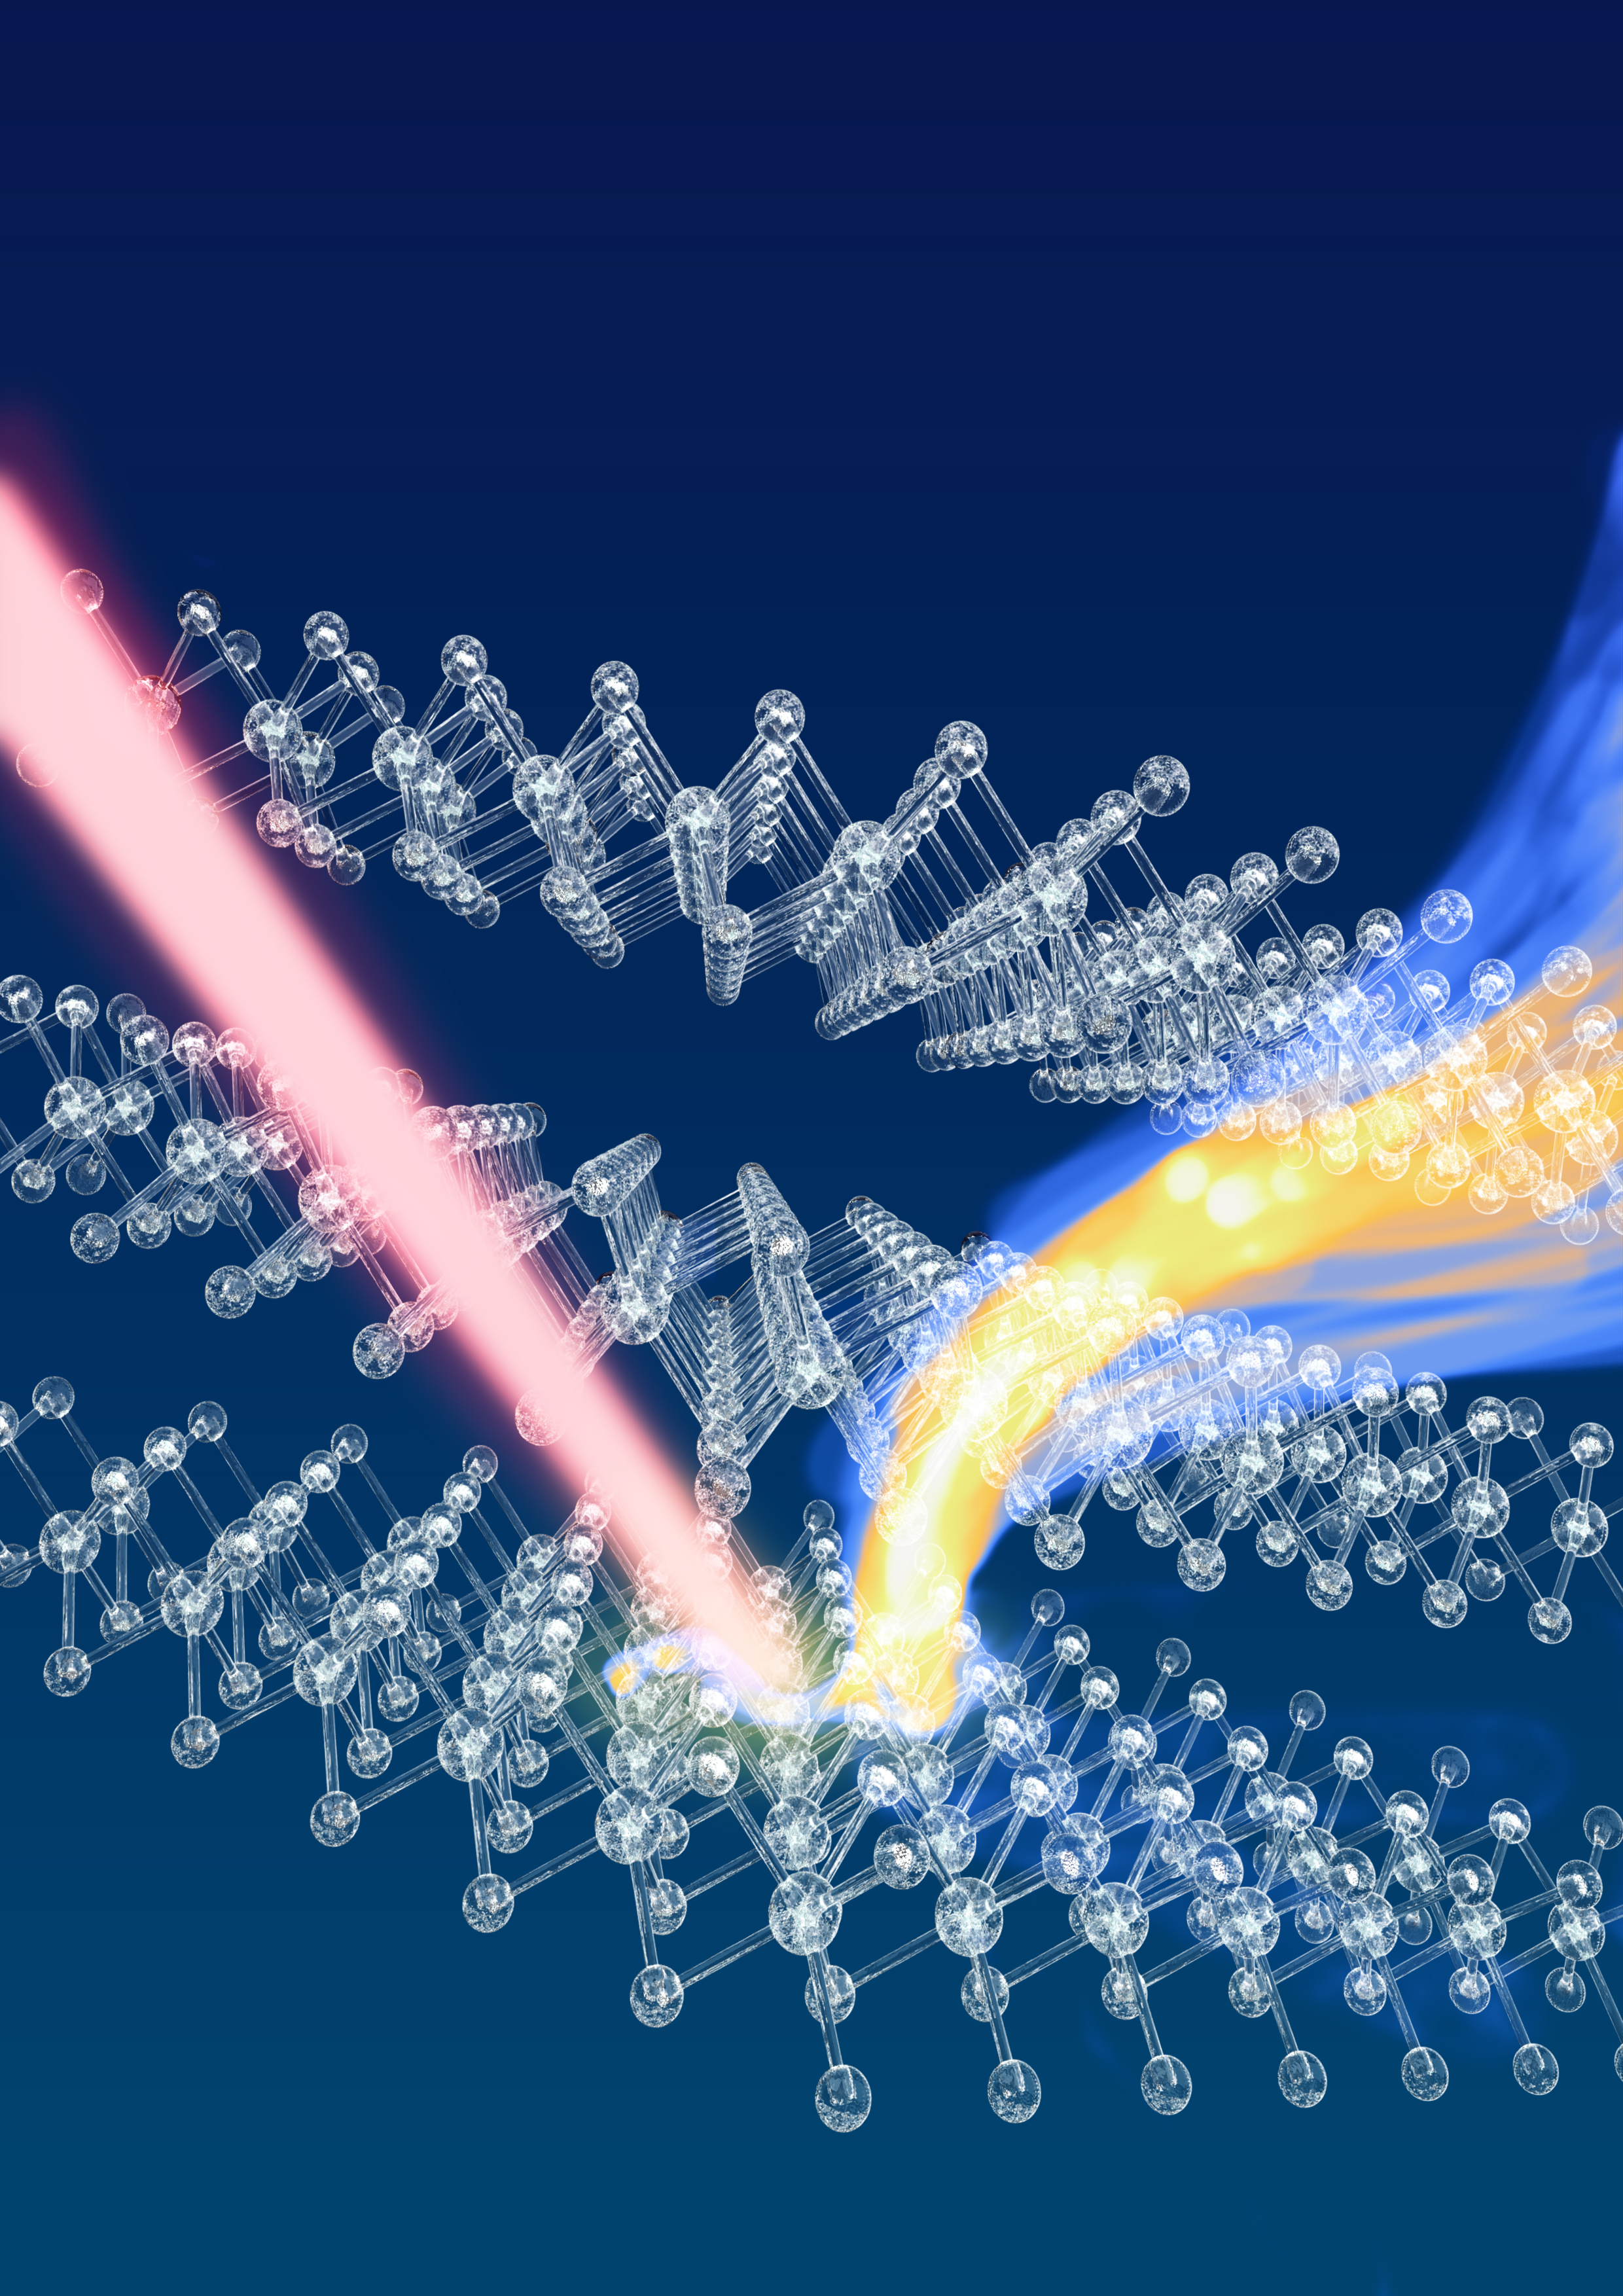
\includegraphics[width=0.6\textwidth]{Figures/Cover_v1.jpg} % 
\end{center}
\end{figure}
\end{quote}
\renewcommand{\baselinestretch}{2}
\small\normalsize

\end{center}
  %(if present, start at lower-case Roman number ii)
 \addcontentsline{toc}{chapter}{Preface}

\phantomsection %create the correct anchor for the bookmark
\addcontentsline{toc}{chapter}{Foreword}
\include{Foreword} %(if present, lower-case Roman)

\phantomsection %create the correct anchor for the bookmark
\addcontentsline{toc}{chapter}{Dedication}
%Dedication

\renewcommand{\baselinestretch}{2}
\small\normalsize
\hbox{\ }
 
\vspace{.5in}

\begin{center}
\large{\textbf{\textit{Dedicated to my grandmother and my parents}}}
\end{center} 


 %(if present, lower-case Roman)

\phantomsection %create the correct anchor for the bookmark
\addcontentsline{toc}{chapter}{Acknowledgements}
%Acknowledgments

\renewcommand{\baselinestretch}{2}
\small\normalsize
\hbox{\ }
 
\vspace{0in}

\begin{center}
\large{Acknowledgments} 
\end{center} 

My PhD journey in UMD is definitely one of the most memorable experience in my life. 
I would like to share my deep appreciation to all the people who helped me along the road. 
This thesis cannot be finished without contributions from them.

At first, I am deeply grateful to my advisor, Prof.You Zhou, 
for his generous support and insightful guidance throughout my PhD. 
As an advisor, he is always patient in answering my questions and provides timely feedback that helps me complete my work efficiently.

I feel truly fortunate to have worked under his supervision, where I learned not only technical skills and knowledge but, equally, integrity and a rigorous attitude toward research.



Your support shaped my approach to research and made this work possible.


\vspace{1ex}


 %(if present, lower-case Roman)
    \cleardoublepage

\phantomsection %create the correct anchor for the bookmark
    \addcontentsline{toc}{chapter}{Table of Contents}
    \renewcommand{\contentsname}{Table of Contents}
\renewcommand{\baselinestretch}{1}
\small\normalsize
\tableofcontents %(required, lower-case Roman)
\newpage

\phantomsection %create the correct anchor for the bookmark
\addcontentsline{toc}{chapter}{List of Tables}
    \renewcommand{\contentsname}{List of Tables}
\listoftables %(if present, lower-case Roman)
\newpage

\phantomsection %create the correct anchor for the bookmark
\addcontentsline{toc}{chapter}{List of Figures}
    \renewcommand{\contentsname}{List of Figures}
\listoffigures %(if present, lower-case Roman)
\newpage

% LIST OF ABBREVIATIONS
\phantomsection %create the correct anchor for the bookmark
\addcontentsline{toc}{chapter}{List of Abbreviations}
\include{Abbreviations-supertabular}

\newpage
\setlength{\parskip}{0em}
\renewcommand{\baselinestretch}{2}
\small\normalsize

%Pages from this point start at Arabic numeral 1
\setcounter{page}{1}
\pagenumbering{arabic}
%Chapter 1

\renewcommand{\thechapter}{1}

\titleformat{\chapter}[display]
  {\bfseries\Huge} % format: bold + large font
  {\chaptertitlename\ \thechapter}{20pt} % "Chapter X"
  {\Huge} % Title itself
\titlespacing*{\chapter}{0pt}{*0}{*4} % adjust spacing above/below

\chapter{Introduction}
\label{chap1}
\section{Overview}
Modern computing is under the combined pressures of scale and efficiency, and AI workloads are growing faster than improvements in transistor density and memory bandwidth\cite{Sun2015-am}.
As models get larger and memory sits farther from the processor, transferring data takes longer and consumes more energy.
Traditional copper interconnects stores charge to send a “1” and discharge to send a “0,” so a longer transfer distance require more energy every time they switch. 
They also respond more slowly because the charge has farther to go and more resistance and capacitance to overcome, which increases latency\cite{Miller2000-lm}.

Optical interconnects can transfer data by encoding electrical signal onto light with on-chip optical modulator,which can avoid Ohmic loss and enable high bandwidth over long distances\cite{Sun2015-am}.
Key building blocks for this consist electro optical modulators, high responsivity photodetectors, compact on-chip light sources(or external input coupling), low-loss waveguides/couplers, and driver electronics\cite{Miller2009-hw,Miller2010-nt}.
Among them, materials such as III–V, LiNbO$_3$, 2D semiconductors provide efficient gain, fast modulation and strong electro-optic effects\cite{Wang2018-ga,Sun2016-gg}.
Among these building blocks, the electro–optic modulator (EOM) is especially critical, as it sets the link bandwidth and energy per bit and largely determines extinction ratio and noise.
The modulation efficiency arises from the material’s nonlinear optical response as function of the electrical field or doping density. 
The induced changes in absorption and refractive index then can convert small electrical drives into large optical contrast. 
In the classical regime, large modulation depth typically requires many photons or high optical fields\cite{Miller2009-hw}. 

2D semiconductors provide strong excitonic behavior which can be easily tuned by the gating voltage. 
This enable the application in ultra compact and low voltage modulator.

Optical computing leverages photons to perform signal processing and computation with intrinsically high bandwidth, low latency, and reduced energy dissipation\cite{Miller2010-nt}. 
Because photons are massless and do not experience resistive losses, optical links can achieve lower energy per bit and avoid the RC bottlenecks that limit charge-based electronics. 

Despite these advantages, a major challenge for all-optical logic is the weakness of optical nonlinearities in conventional materials\cite{Boyd2020-re}. 
Since photons do not interact in linear media, and inducing a significant optical response typically requires high field intensities or large photon numbers\cite{Chang2014-hk}. 
Current optical switches based on the Kerr effect or free carrier modulation require elevated power levels for fast modulation, leading to effects such as two-photon absorption, excess carrier and heat generation\cite{Miller2009-hw}.
These side effects inject noise and cause thermal drift, especially when many devices are integrated on the same chip.

A promising path forward is to enter the quantum nonlinear regime, where even a few photons can interact strongly. 
One key goal is to achieve photon blockade, in which the presence of a single photon shifts the system energy to prevent the entry of a second\cite{Imamoglu1997-pb}. 
This enables single photon switches, quantum logic gates, and generation of nonclassical light source, all essential components for scalable quantum photonic circuits\cite{Lodahl2015-el,Chang2014-hk}. 
However, realizing photon blockade requires nonlinear energy shifts that exceed the linewidth\cite{Carusotto2013-mf}. 

Photon blockade requires anharmonic shift $U \geq \Gamma$, where $\Gamma=\kappa+\gamma^\ast$ is the total linewidth including cavity decay $\kappa$ and pure dephasing $\gamma^\ast$~ \cite{Birnbaum2005-ix,Verger2006-jz}. 
For a Kerr medium, the $U$ is proportional to $g /A_{\mathrm{eff}}$, where $g$ is a property from the material nonlinear coupling. $A_{\mathrm{eff}}$ the optical mode area. 
In standard dielectric or III–V cavities, one typically finds $g \sim 0.1$–$1~\mu\mathrm{eV}\cdot\mu\mathrm{m}^2$ and $A_{\mathrm{eff}}\sim 5$–$20~\mu\mathrm{m}^2$.
This gives out an overall $U\sim 0.01$–$0.2~\mathrm{meV}$, which is usually below $\Gamma\sim 0.2$–$2~\mathrm{meV}$ even at cryogenic temperatures. 
That's why it's challenging in realizing this in conventional materials or systems.

2D semiconductors offer a unique opportunity to bridge this gap. 
Their tightly bound excitons exhibit large oscillator strengths and support strong exciton exciton interactions, giving rise to large Kerr-like optical nonlinearities\cite{Wang2018-qm}. 
These interactions can be further enhanced by coupling to optical cavities\cite{Datta2022-po,Walther2018-jp}, engineering moiré potentials\cite{Zhang2021-eb}, or applying spatial confinement\cite{Thureja2022-yc}, pushing device operation into the few-photon regime. 
The atomically thin nature of 2D materials enables ultra compact devices and high density integration via van der Waals stacking, compatible with silicon photonics and CMOS platforms\cite{de-Abajo2025-vm}. 
Moreover, gate tunable carrier densities and valley control offer additional knobs to optimize modulation speed, contrast, and noise\cite{Mak2012-le}. 
The intrinsically short radiative lifetime of excitons\cite{Wang2018-zb}, while challenging for photon statistics measurements, are advantageous for creating single-photon sources with high repetition rates and ultrafast optical switches\cite{Korzh2020-ya,Esmaeil-Zadeh2020-mp}. 

In summary, no matter for classical and quantum nonlinear optics applications, enhancing the interaction strength among optical excitations and reducing their linewidth are critical goals.
While challenges remain in materials growth, theoretical understanding and device engineering, the outlook for 2D materials in nonlinear optics is overwhelmingly positive. 
Their properties coupled with ongoing innovations, position them as transformative building blocks for the next generation of optical technologies. 

\section{Thesis Outline}
This thesis focus on developing systems with large exciton interactions towards giant optical nonlinearity.
Chapter~\ref{chap2} will discuss the background of excitons, exciton-polaritons and the related physics about TMD semiconductors. 
Chapter~\ref{chap3} will introduce the experimental and numerical methods applied through the thesis.
Chapter~\ref{chap4} will discuss the approach towards exciton quantum confinement with novel electrostatic superlattice.
Chapter~\ref{chap5} will introduce the developed system with giant optical nonlinearity of Fermi polarons, where the exciton-carrier interaction contributes to this large nonlinear shift.
Chapter~\ref{chap6} will discuss the ongoing project based on Chap.~\ref{chap5} that we leverage cavity engineering for realizing polaron-polariton with enhanced optical nonlinearity.
Chapter~\ref{chap7} summarize the whole thesis and discuss the future directions of the work.



%%Chapter 2

\renewcommand{\thechapter}{2}

\chapter{Background of the system}

\section{Basic structure of 2D Transition Metal Dichalcogenides}

\subsection{Lattice Structure}
Transition metal dichalcogenides(TMD) semicondcutor have the general chemical formula of $MX_2$, where $M$ refers to the transition metal atom($Mo,W$) and $X$ is the chalcogen atom($S$,$Se$,$Te$).
In the TMD bulk crystal, the metal and chalcogen atoms are bonded through covalent-ionic bonds, whereas different layers are bonded by the weak van der Waals force.
This enables accessing the monolayer TMD through mechanical exfoliation.
There are three different phases in the TMD crystal: hexagonal 2H, rhombohedral 3R, and trigonal 1T' phases. In their most thermaldynamic stable phase 2H polytype, a monolayer consists of a hexagonal plane of transition metal atoms sandwiched between two planes of chalcogen atoms, forming trigonal prismatic coordination.
This yields a honeycomb-like lattice with \textbf{$D_{3h}$} 
point-group symmetry at the monolayer level, with the absence of inversion symmetry. 
However, this inversion symmetry can be restored in even number multilayers, with one layer is rotated $180^\circ$ relative to the other layer.

In 3R phase, each successive monolayer is shifted relative to the one below, following an ABC stacking order and belongs to the \textbf{$C_{3v}$}point group rather than the AB sequence of the 2H phase. 
This stacking is characterized by the absence of inversion symmetry at all thicknesses. 
As a result, strong second-order nonlinear optical processes, such as second-harmonic generation, have been extensively investigated in 3R multilayers\cite{Xu2022-at,Qin2024-xt}.

The 1T phase, by comparison, features octahedral coordination of the transition-metal atoms with $D_{3d}$ point-group symmetry, which includes inversion symmetry even at the monolayer level.
While the ideal 1T structure is metallic, certain compounds undergo lattice distortions into the so-called 1T$^{\prime}$ phase, which breaks inversion symmetry and can host semimetallic or topologically nontrivial states, including quantum spin Hall insulators and type-II Weyl semimetals.
%%figure1-1
\renewcommand{\baselinestretch}{2}
\small\normalsize
\begin{quote}
\begin{figure}
\begin{center}
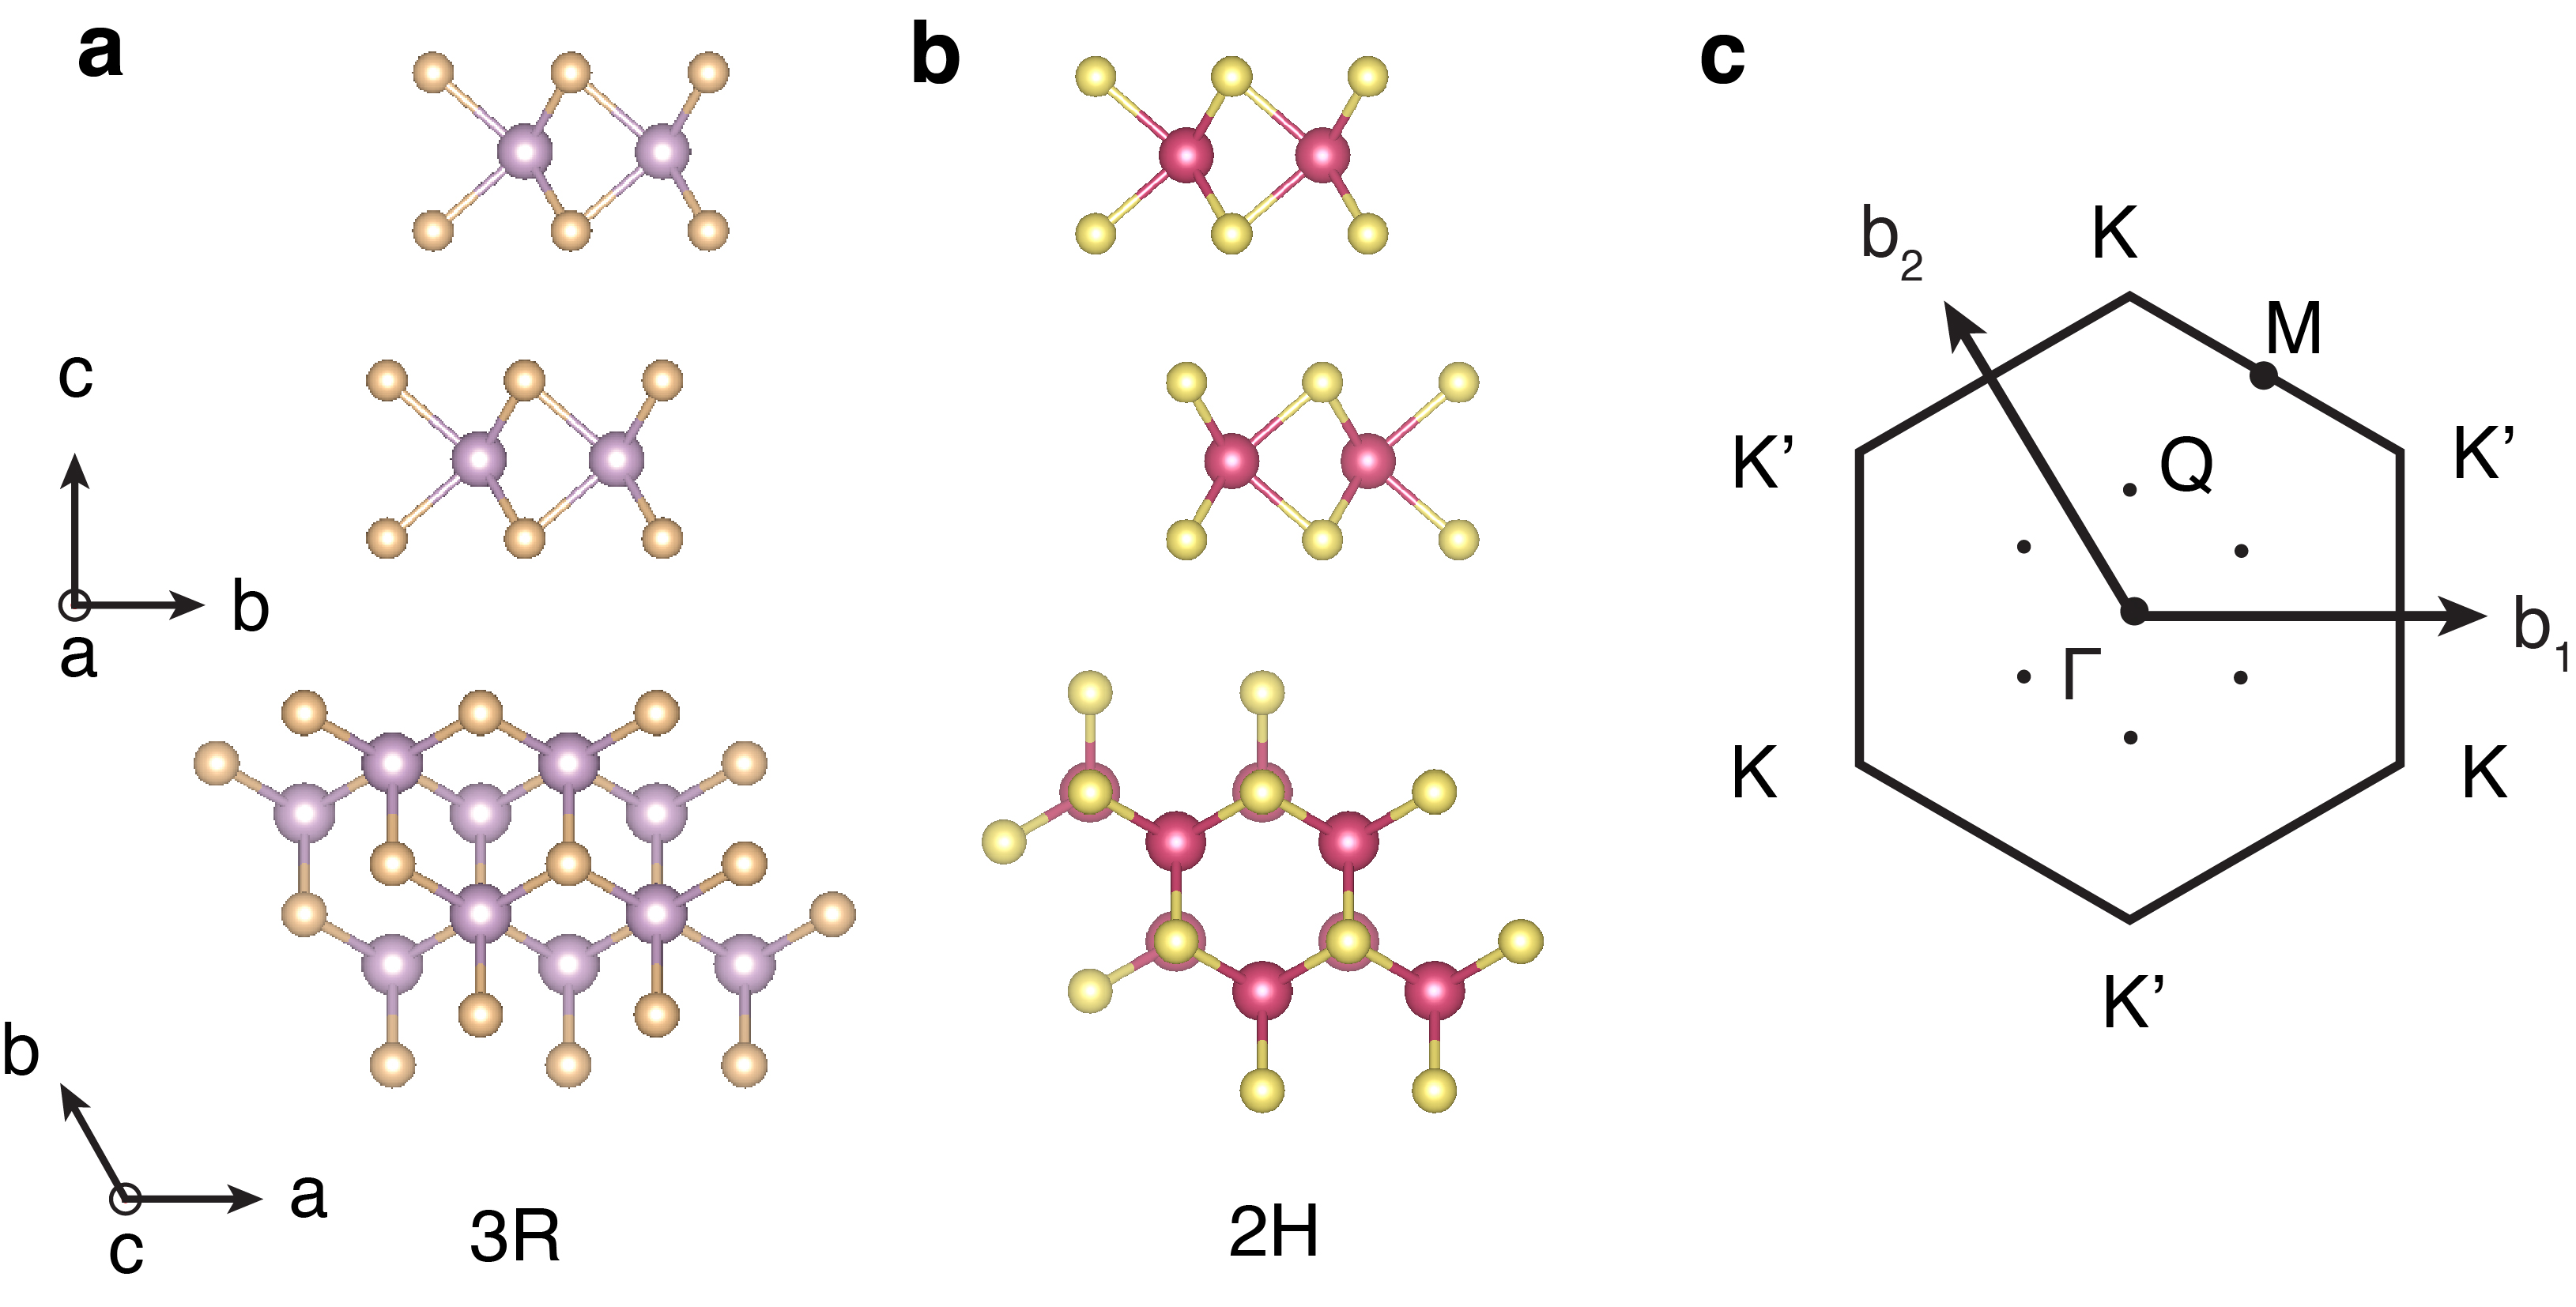
\includegraphics[width=0.85\textwidth]{Figures/C2/Fig.2-1_lattice.jpg}%
\end{center}
\caption[\textbf{Crystal structures of TMDC.}]{\textbf{a,b,} Side view (top) and top view (bottom) of the 3R and 2H stacking structure. 
\textbf{c,} Hexagonal Brillouin zone of TMD with the reciprocal lattice vectors $\mathbf{b_1}$ and $\mathbf{b_2}$.}
\label{fig.lattice}
\end{figure}
\end{quote}
\renewcommand{\baselinestretch}{2}
\small\normalsize
% ------

\subsection{Electronic band structure of TMD}
In this thesis, we mainly study the layers mechanically exfoliated from 2H phase TMD. The discussion of the electronic bandstructure would thus mainly focus on the 2H phase. 

For the semicondcutor TMDCs, the bandgap is around 1 to 2 eV\cite{Manzeli2017-nt}.
In the monolayer TMD, the conduction band minimum and valence band maximum located at the corner of the Brillouin zone $K$ ($K^\prime$) valley, which is mainly derived from the transition-metal $d$ orbitals ($d_{z^2}$ for the conduction band and $d_{x^2-y^2}$ + $d_{xy}$ for the valence band)\cite{Liu2013-jh}. 
%%figure1-2
\renewcommand{\baselinestretch}{2}
\small\normalsize
\begin{quote}
\begin{figure}
\begin{center}
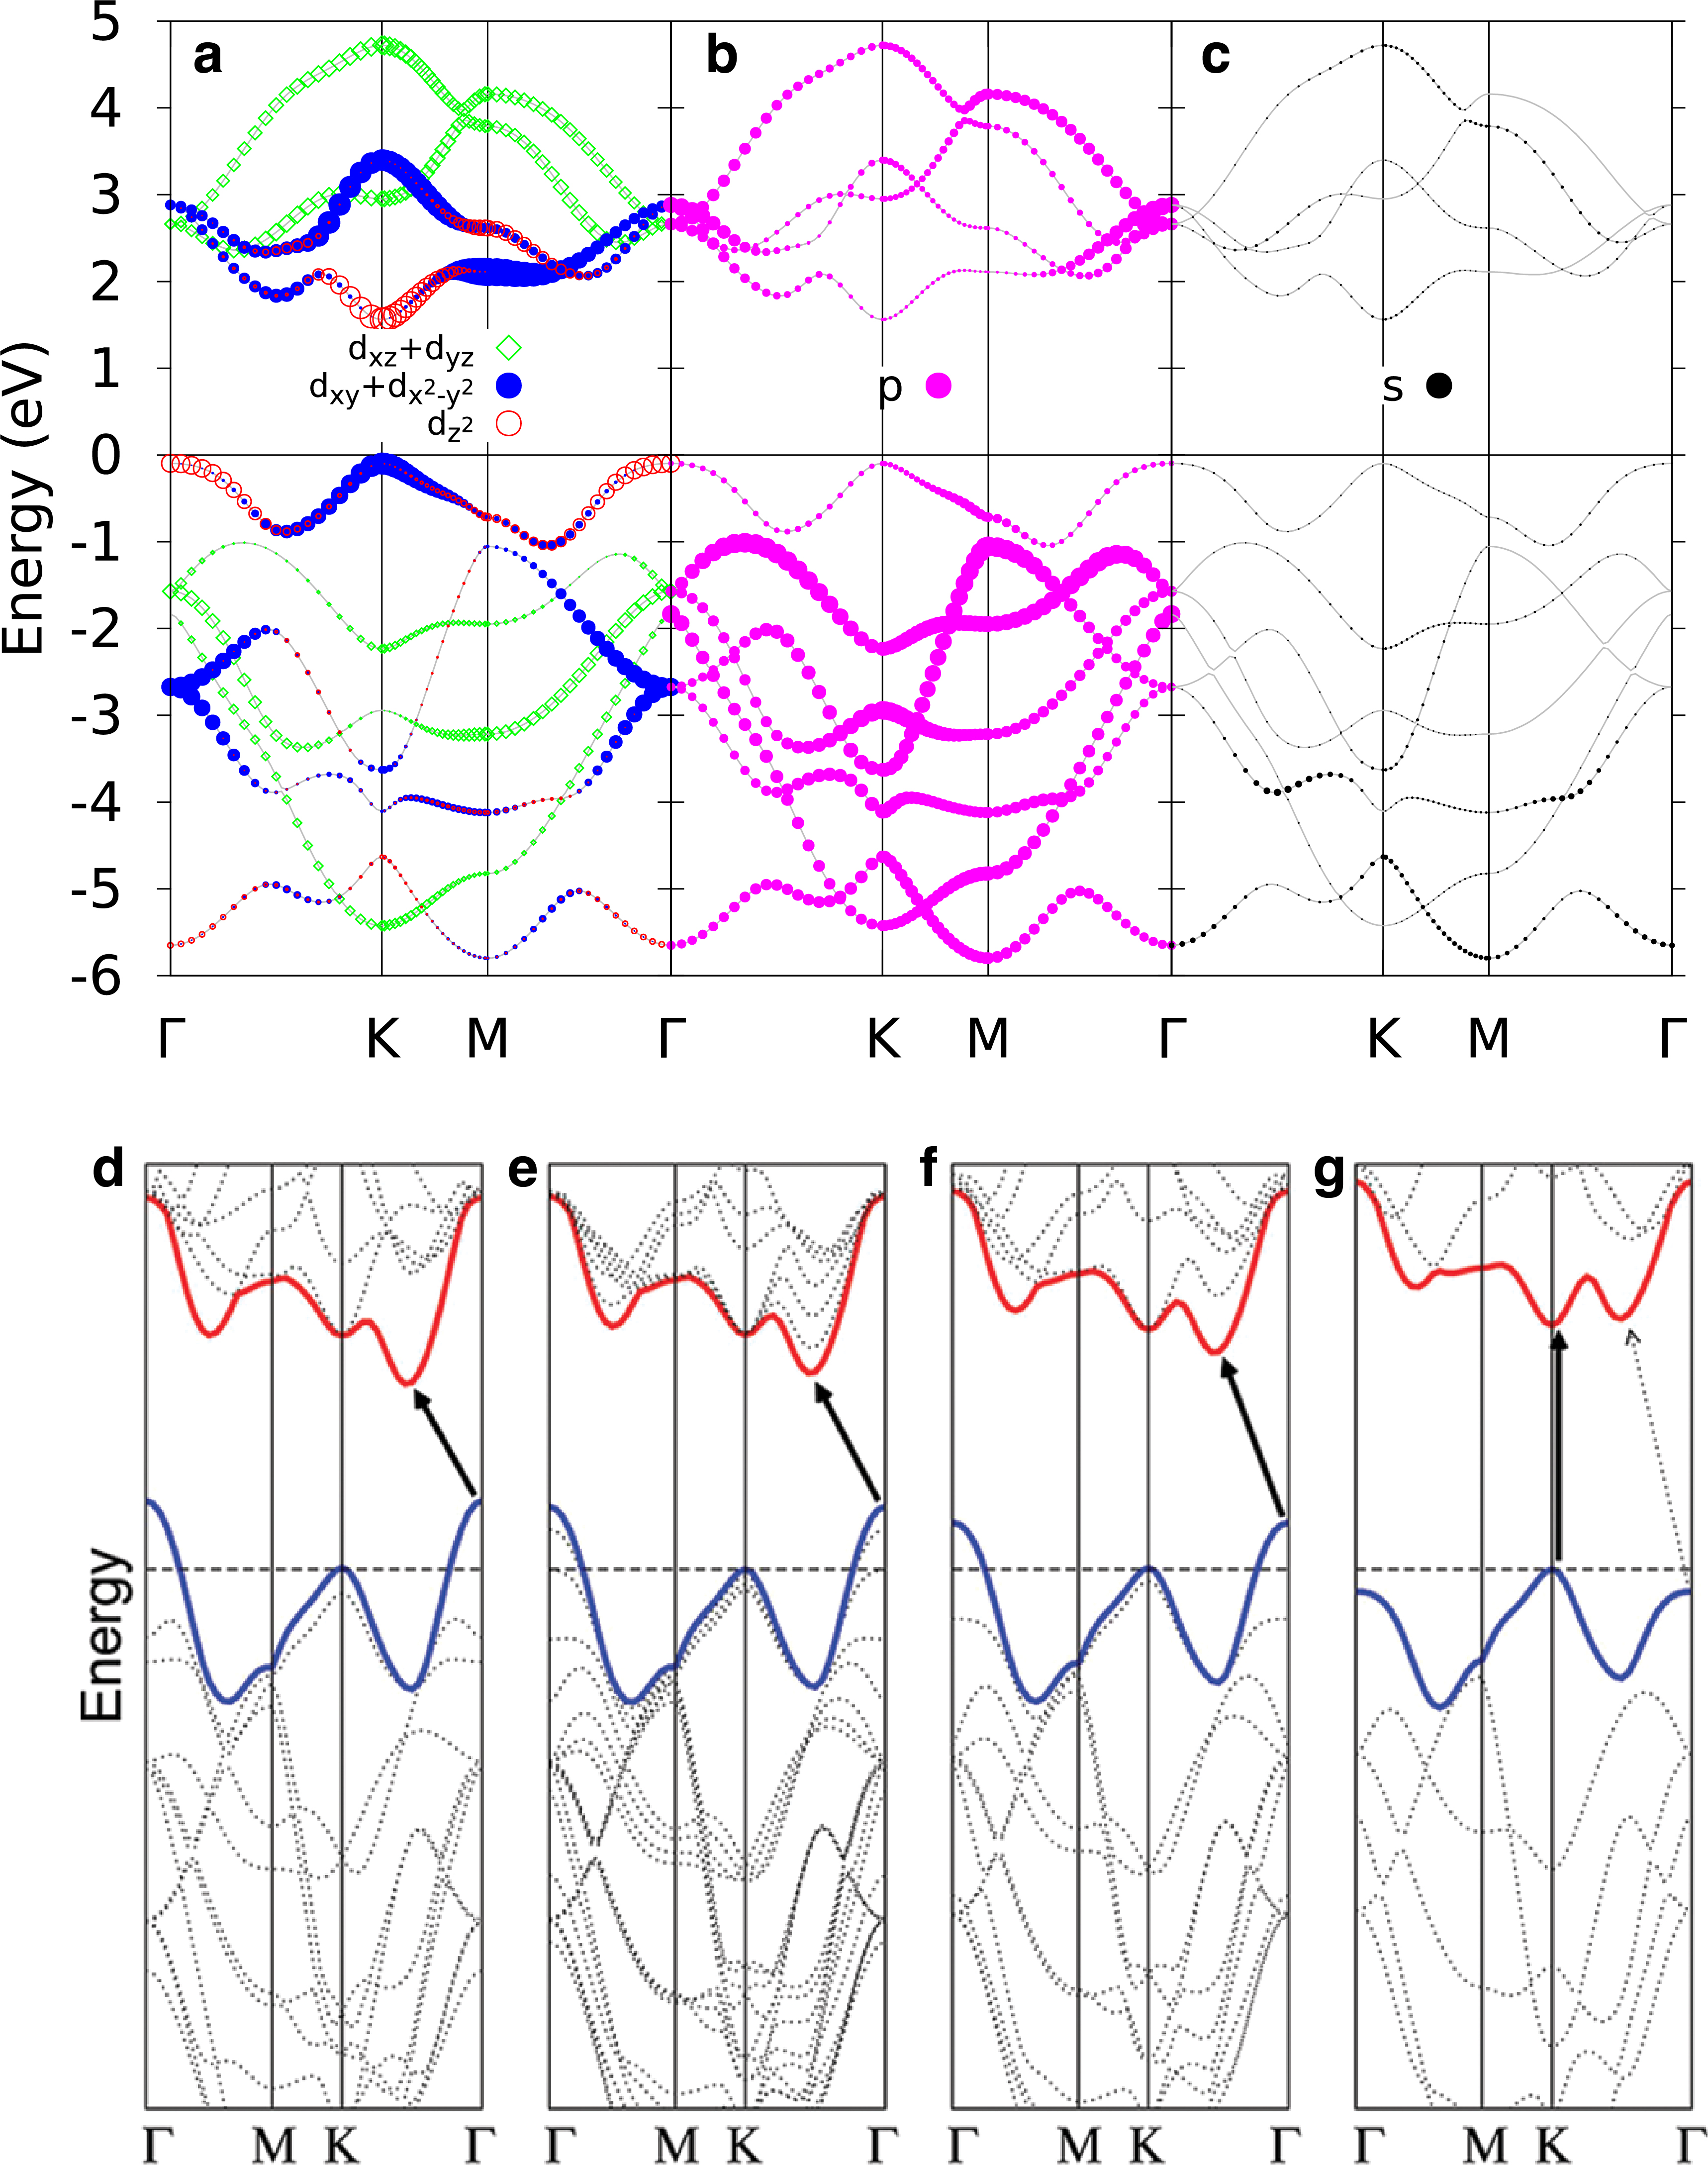
\includegraphics[width=0.65\textwidth]{Figures/C2/Fig.2-2_bandstructure.jpg}%
\end{center}
\caption[\textbf{Band structures of TMDC.}]{\textbf{a,b,c} Calculated orbital projected band structure for monolayer $MoS_2$, with \textbf{a} contribution from the Mo atom $d$ orbitals;\textbf{b}Total $p$ orbitals dominated by the chalcogen S atom; \textbf{c} Total $s$ orbital.
\textbf{d,e,f,g} Calculated bandstructure of bulk,quadrilayer,bilayer and monolayer TMD(from left to right).
The crossover from indirect to direct bandstructure happens at the monolayer limit.Figure adpated from\cite{Splendiani2010-km,Liu2013-jh}.}
\label{fig.band}
\end{figure}
\end{quote}
\renewcommand{\baselinestretch}{2}
\small\normalsize

One well-known feature of the TMD materials is the indirect to direct band structure transition when the layer thickness is approaching to the monolayer limit\cite{Mak2010-dq}.
This crossover arises from the different sensitivity of electronic states at distinct wave vectors to interlayer coupling and quantum confinement\cite{Splendiani2010-km}.
At the k points, states are strongly localized around the metal atoms and therefore remain largely unaffected by interlayer coupling. 
In contrast, the valence states near $\Gamma$ and the conduction states near the $Q$ valley (between $\Gamma$ and $K$) originate from hybridization between transition-metal $d$ orbitals 
and chalcogen $p_z$ orbitals. 
Because the $p_z$ orbitals extend out of plane, they are more 
delocalized and thus highly sensitive to interlayer coupling. 
As a result,with increasing layer numbers lifts the $\Gamma$ valence band upward and lowers the $Q$ conduction band, while the $K$ valleys remain nearly unchanged.
Figure~\ref{fig.band} shows this direct–indirect crossover in the calculated bandstructures.

\subsection{Spin-orbit interaction}
Spin--orbit coupling (SOC) arises from the relativistic interaction between an electron’s orbital motion and its spin. 
In the effective one-electron picture, the SOC Hamiltonian can be expressed as
\begin{equation}
H_{\mathrm{SOC}} = \xi(r)\, \mathbf{L}\cdot\mathbf{S}
\label{eq.SOC}
\end{equation}
where $\mathbf{L}$ and $\mathbf{S}$ are the orbital and spin angular momenta, and $\xi(r)$ denotes the radial SOC strength, which increases strongly with atomic number\cite{Sakurai2020-jh,Winkler2003-ty}. 
In transition-metal dichalcogenides (TMDs), the heavy transition-metal atoms (Mo, W) provide a strong SOC environment that directly impacts the band edges\cite{Xiao2012-pw,Liu2013-jh}.
At the $K$ and $K'$ valleys, the valence-band maximum is primarily derived from in-plane $d_{x^2-y^2}$ and $d_{xy}$ orbitals. 
In the complex orbital basis, these states correspond to magnetic quantum numbers $m_l = \pm 2$, which carry significant angular momentum around the $z$-axis. 
Their strong coupling to spin through the $L_z S_z$ interaction results in a large spin splitting, typically several hundred meV, especially for W-based TMD\cite{Kormanyos2015-dn,Zhu-Z-Y-and-Cheng-Y-C-and-Schwingenschl-ogl-U2011-lo}.
In contrast, the conduction-band minimum originates mainly from the $d_{z^2}$ orbital ($m_l = 0$), which carries zero orbital angular momentum projection along $z$. 
However, the calculation of the bandstructure shows a finite spin splitting in the value of a few meV in the conduction band.
This arises through SOC-mediated coupling of the 
$d_{z^2}$ state to nearby orbitals that carry finite angular momentum ($m_l = \pm 1$), most importantly the transition-metal $d_{xz}/d_{yz}$ and chalcogen $p_x/p_y$ states\cite{Liu2013-jh,Kosmider2013-bt}. 
In MoX$_2$, this interaction produces a negative splitting, so the lower conduction subband has the opposite spin orientation to the valence-band maximum. 
In contrast, WX$_2$ compounds exhibit a positive splitting, and the conduction subband ordering is reversed\cite{Liu2013-jh}.
The broken inversion symmetry together with strong spin–orbit coupling in monolayer TMDs gives rise to spin–valley coupling, which enables control of valley degrees of freedom through phenomena such as the valley Hall effect and valley-selective optical transitions\cite{Mak2012-le,Cao2012-tt,Xiao2012-pw}.

\subsection{Valley-Dependent Optical Selection Rules}
Optical transitions in semiconductors are governed by the electric-dipole selection rule, 
which enforces conservation of angular momentum between the electron system and the absorbed or emitted photon\cite{Yu2010-yp,Fox2010-ly}. 
The corresponding transition amplitude can be written as\cite{Fox2010-ly}:
\begin{equation}
M_{\pm}(\mathbf{k}) = \big\langle \psi_{c}(\mathbf{k}) \big| 
\hat{\mathbf{p}} \cdot \mathbf{e}_{\pm} 
\big| \psi_{v}(\mathbf{k}) \big\rangle,
\label{eq.OP transition}
\end{equation}
where $\psi_{v}$ and $\psi_{c}$ denote the valence- and conduction-band Bloch states,
$\hat{\mathbf{p}}$ is the momentum operator, and
$\mathbf{e}_{\pm} =\frac{1}{\sqrt{2}} (\hat{x} \pm i\hat{y})$ are polarization vectors for right- ($\sigma^{+}$) and left- ($\sigma^{-}$) handed circularly polarized light\cite{Teich1991-lv}.
Because $\mathbf{e}_{\pm}$ carries angular momentum projection $\pm \hbar$ along the light propagation axis, a circularly polarized photon transfers angular momentum $\pm 1$ into the electronic system\cite{Fox2010-ly}. 
Thus, optical excitation with $\sigma^+$ or $\sigma^-$ light can
be used to probe states that differ in their orbital angular momentum by one unit\cite{Cao2012-tt,Xiao2012-pw,Mak2012-le}.

In semiconducting TMD monolayers, the broken inversion symmetry and strong spin--orbit coupling translate these general rules into valley-specific selection rules\cite{Xiao2012-pw}. 
The valence band maximum at the inequivalent $K$ and $K'$ valleys is dominated by metal $d_{x^2-y^2}$ and $d_{xy}$ orbitals, which combine as $d_{x^2-y^2} \pm i d_{xy}$ and carry angular momentum projections $m_l = \pm 2$.
The conduction band minimum is mainly derived from the $d_{z^2}$ orbital ($m_l=0$)\cite{Liu2013-jh}. 
Interband optical transitions are therefore allowed only if the angular momentum of the photon compensates the orbital character of the valence state. 
As a consequence, transitions at the $K$ valley couple exclusively to $\sigma^+$ photons, while those at $K'$ couple only to $\sigma^-$ photons as shown in Figure~\ref{fig.selection-rule}.

%Fig.5--------------
\renewcommand{\baselinestretch}{1}
\small\normalsize
\begin{quote}
\begin{figure}
\begin{center}
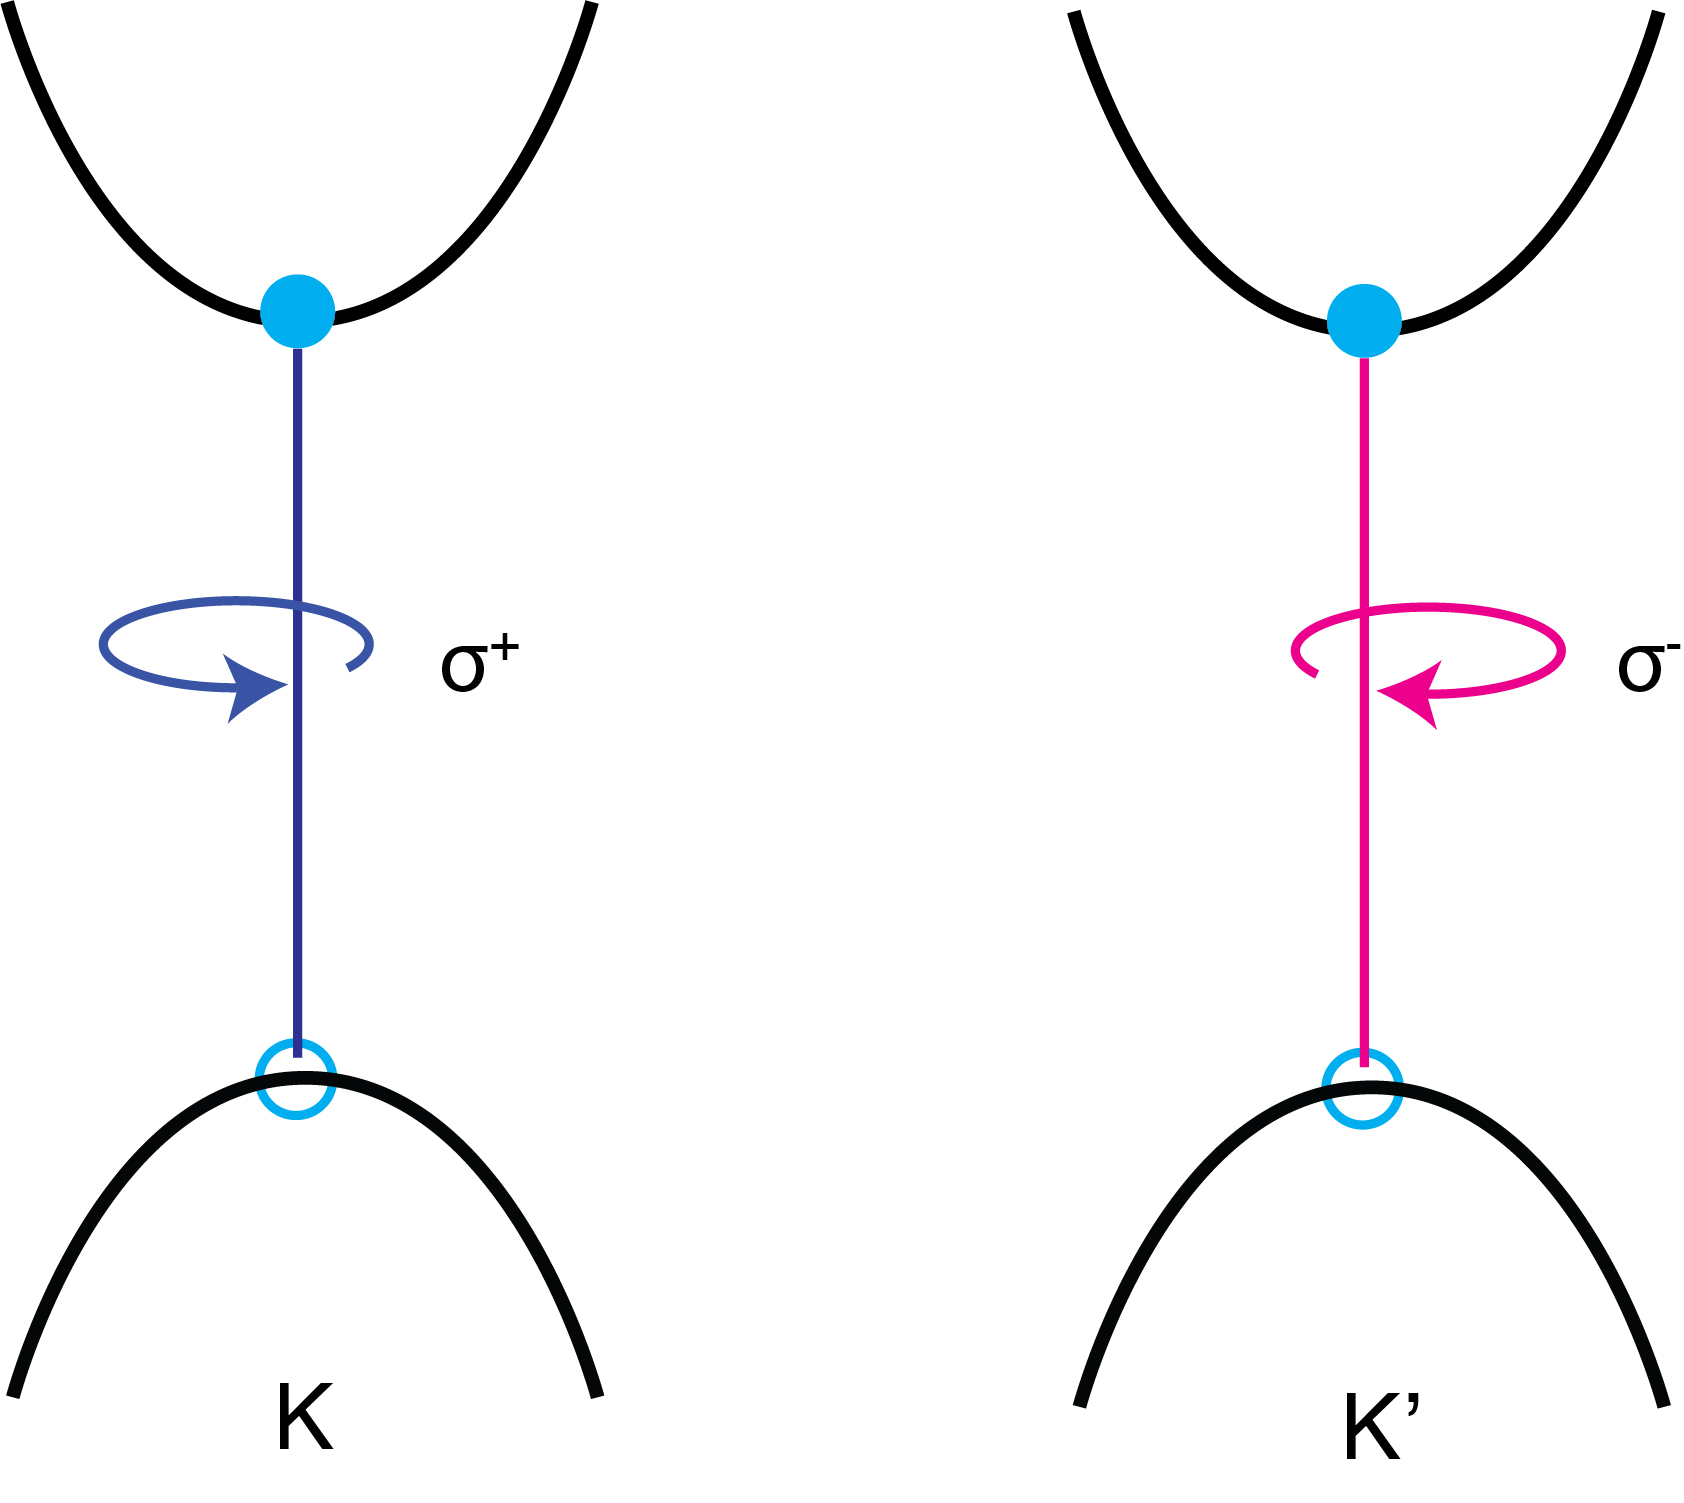
\includegraphics[width=0.4\textwidth]{Figures/C2/Fig.selection_rule.jpg} % 
\end{center}
\caption[Valley-dependent optical selection rule] {\textbf{Valley-dependent optical selection rule.}The left and right circular polarized light coupled to the $K$ and $K^\prime$ valley, respectively.}
\label{fig.selection-rule}
\end{figure}
\end{quote}
\renewcommand{\baselinestretch}{2}
\small\normalsize
% --------------
This valley--helicity locking gives rise to valley-selective circular dichroism, as demonstrated in monolayer MoS$_2$ \cite{Mak2012-le,Zeng2012-ss}. 
The experimental observation of nearly perfect polarization selectivity provides direct evidence that inversion symmetry
breaking is essential for lifting valley degeneracy in optical transitions.

However, in bilayer TMDs with 2H stacking, where the top layer is rotated by $180^{\circ}$ relative to the bottom layer, the inversion
symmetry is restored, and the valley-dependent optical selection rules are lost: both valleys can now couple to both helicities with equal weight. 
As a result, bilayer MoS$_2$ shows no net circular dichroism under optical excitation \cite{Mak2012-le}. 
This striking contrast between monolayer and bilayer systems highlights the crucial role of symmetry:
broken inversion symmetry in monolayers enforces a one-to-one correspondence between photon helicity and valley index, while the restoration of inversion symmetry in bilayers removes this correspondence and suppresses valley polarization.

In summary, the valley-contrasting optical selection rules in monolayer TMDs originate from the unique orbital composition of the band edges and the absence of inversion symmetry. 
These rules form the microscopic basis of valley-selective optical excitation and detection, establishing light helicity as a powerful handle to manipulate valley degrees of freedom in two-dimensional semiconductors\cite{Yu2017-jb}.

\section{Excitons in TMDs}
When the semiconductor absorbs a photon with energy greater than its band gap, an electron would be promoted from the valence band to the conduction band and leaves a positively charged hole in the valence band. 
The Coulomb attraction between the negatively charged electron and the hole can lead to the formation of a bound electorn-hole pair called exciton\cite{Fox2010-ly,Yu2010-ae}. 

Excitons can be classified into two types depending on the spatial extent of the electron--hole wavefunction. 
Frenkel excitons, typically exist in molecular crystals and insulators, are tightly bound and localized on the scale of one unit cell. 
In contrast, Wannier–Mott excitons have a larger radius and extend over many unit cells, so their center of mass can propagate through the crystal. 
Owing to this spatial delocalization, they are commonly referred to as free excitons.

\subsection{Wannier equation and binding energy}
The energy of the exciton can be obtained by solving the two-body Schrödinger equation, which can be written in relative and center-of-mass coordinates. 
The relative motion based on the effective mass can be described by the Wannier equation\cite{Yu2010-ae}:
\begin{equation}
-\left[ \frac{\hbar^2}{2\mu} \nabla^2 + V(\textbf{r}) \right] \psi_{n}(\textbf{r}) 
= E_{n} \, \psi_{n}(\textbf{r})
\label{eq:wannier}
\end{equation}
where $\mu =\frac {m_e m_h}{(m_e+m_h)}$ is the reduced mass,$\psi_{n}(r)$ is the exciton wavefunction. $V(r)$ is the Coulomb interaction, and $E_n$ are the excitonic eigenenergies below the band gap $E_g$. 
$V(r)$ has the Coulomb form as:
\begin{equation}
V(\textbf{r}) = - \frac{e^2}{4\pi \varepsilon_0 \varepsilon_r \textbf{r}}
\label{eq:coulomb}
\end{equation}
By solving the Wannier equation with 3D and 2D Laplace operator in polar coordinates, we can obtain the exciton binding energies follow a Rydberg series\cite{Chernikov2014-vo,Yu2010-ae}:
\begin{flalign}
E_{B,3D}^{(n)} = - \frac{R_X}{n^2} \quad n = 1,2,3,\dots \\[6pt]
E_{B,2D}^{(n)} = - \frac{R_X}{(n-\frac{1}{2})^2},\quad n = 1,2,3,\dots 
\label{eq:exciton_rydberg}
\end{flalign}
$n$ is the principal quantum number, $E_{B,3D}^{(n)}$ is the exciton binding energy in three dimension and $E_{B,2D}^{(n)}$ is the binding energy in 2D plane.$R_X$ is the exciton Rydberg energy and can be expressed as 
$R_X = \frac{\mu}{m_0\varepsilon_r^2}R_H$. $R_H$ is the Rydberg energy of the hydrogen atom(13.6 eV). $\mu$ refers to the reduced electron--hole mass and $\varepsilon_r$ is the relative dielectric
constant. 
The exciton binding energy and the electronic band gap would have the relationship shown as:
\begin{equation}
E_n = E_g-E_{B,2D/3D}^{(n)}
\label{eq:optical gap}
\end{equation}\vspace{-0.5em}
where $E_g$ is the quasiparticle band gap, $E_n$ is the optical band gap when $n =1$. The corresponding exciton Bohr radius for the 1S exciton in 3D and 2D can be obtained as:
\begin{align}
a_{B,3D} &= \frac{4\pi \varepsilon_0 \varepsilon_r \hbar^2}{\mu e^2} 
           = a_0 \cdot \frac{\varepsilon_r}{\mu/m_0} \\[6pt]
a_{B,2D} &= \frac{2\pi \varepsilon_0 \varepsilon_r \hbar^2}{\mu e^2} 
           = a_0 \cdot \frac{\varepsilon_r}{2\mu/m_0} 
           = \frac{1}{2} a_{B,3D}
\label{eq:exciton_bohr_radius}
\end{align}
The $a_0$ value refers to the atomic Bohr radius. 
Compared to the 3D case, the 1s exciton confined to a 2D plane exhibits a binding energy that is enhanced by a factor of four.
This can be understood that when the dimensionality is reduced from 3D to 2D, the exciton cannot spread out in all three spatial directions.
Instead, the electron and hole are forced to remain in the same plane, which increases their spatial overlap. 
This increased overlap enhance the Coulomb attraction, leading to a smaller Bohr radius and larger binding energy in the 2D plane.
In real experiments, TMDs are typically studied in device structures encapsulated by dielectric hBN to prevent any inhomogeneous perturbation,and it has a relatively low permittivity of about 3\cite{Hunt2013-ma}.
This weak screening further enhances the Coulomb interaction, resulting in a much larger exciton binding energy($\sim$ 500 meV)\cite{Wang2018-my} compared to that in GaAs quantum wells($\sim$ tens of meV)\cite{Nakwaski1995-hc}.

%Fig.1-4--------------
\renewcommand{\baselinestretch}{1}
\small\normalsize
\begin{quote}
\begin{figure}
\begin{center}
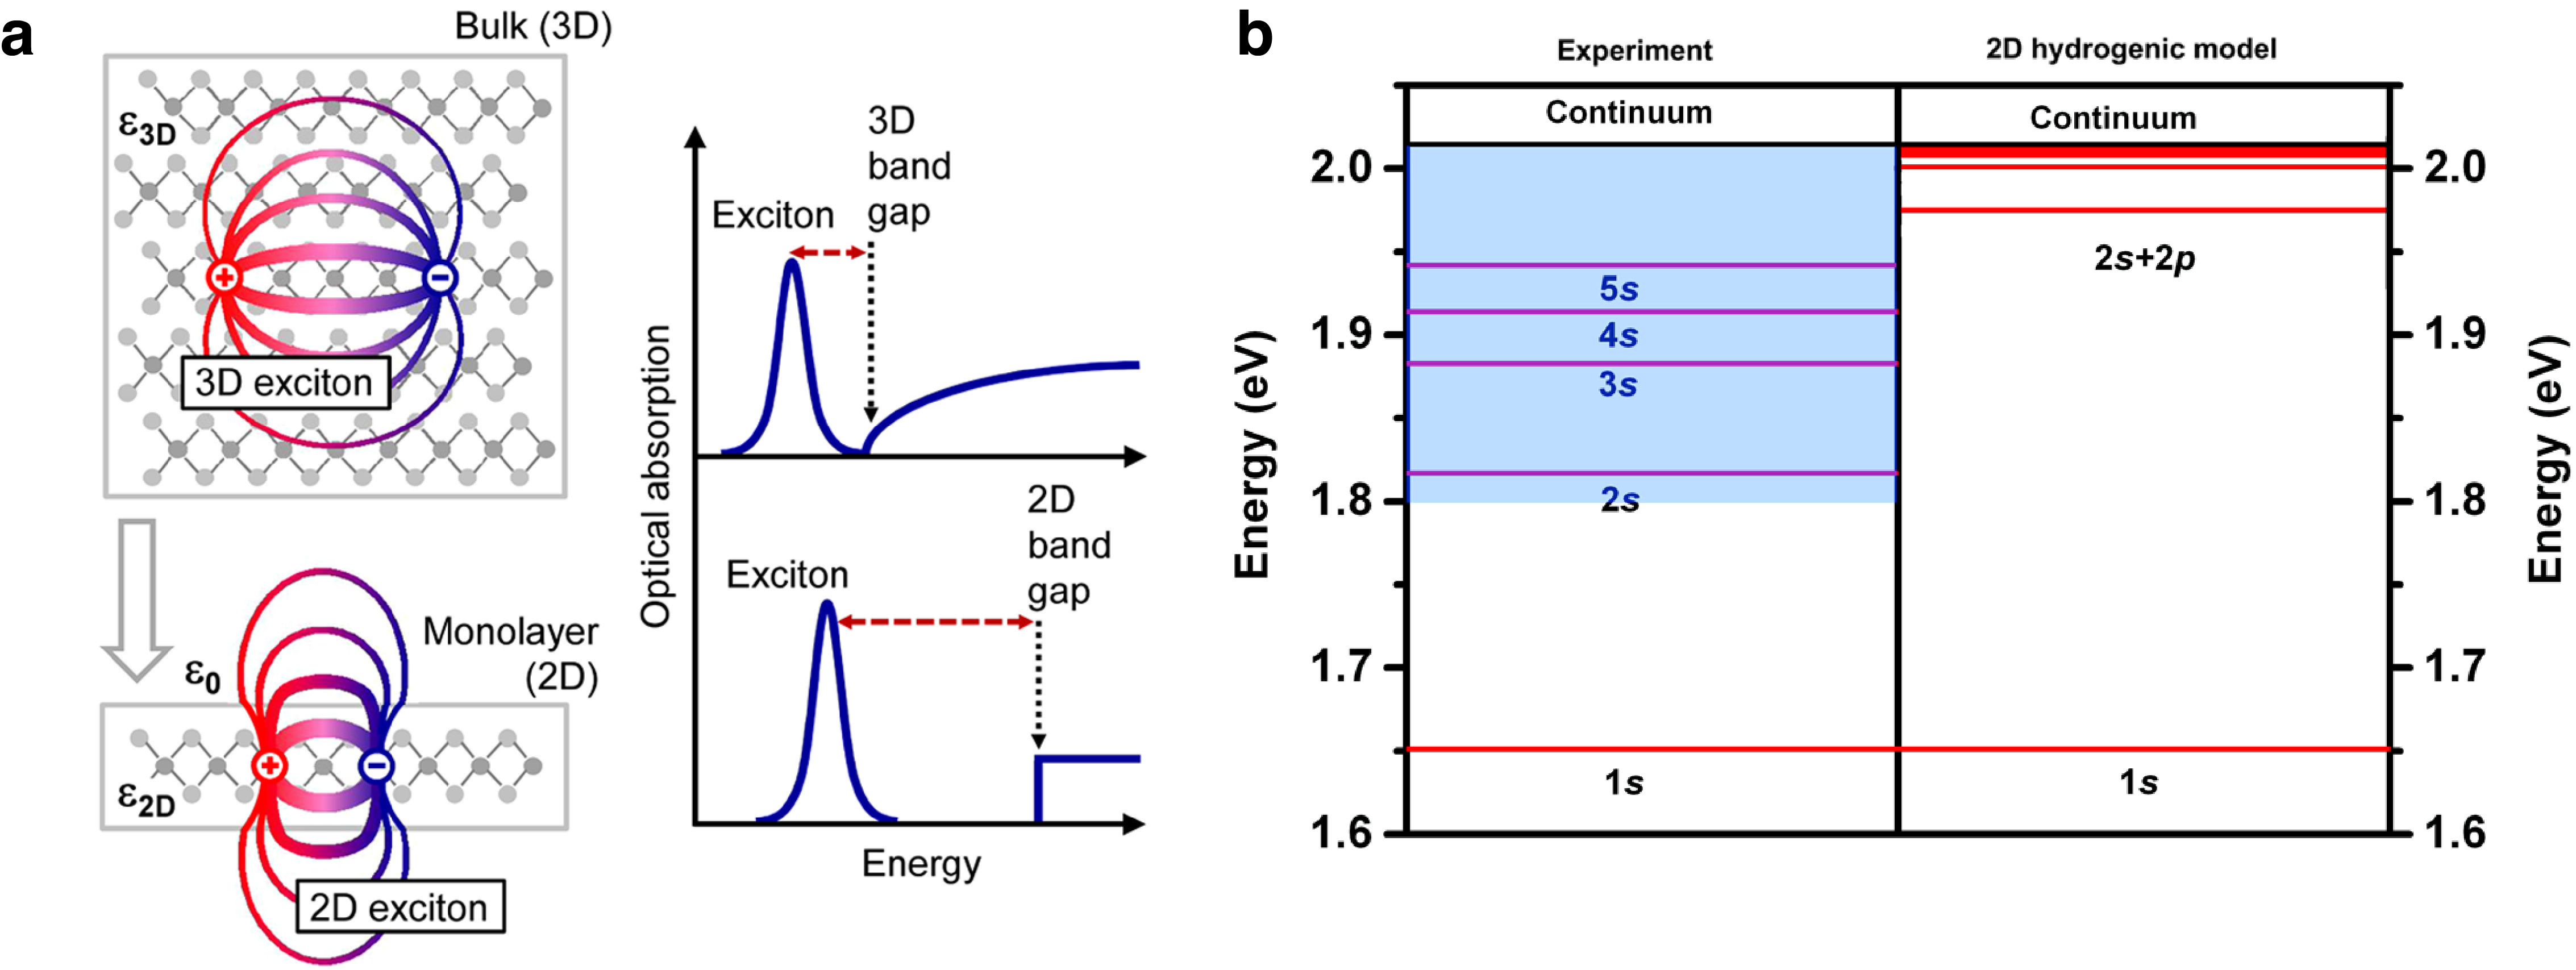
\includegraphics[width=1\textwidth]{Figures/C2/Fig.2-4_rydbergEx.jpg} 
\end{center}
\caption[Rydberg exciton states in 2D TMDCs] {\textbf{Rydberg exciton states in 2D TMDCs.} \textbf{a,}Schematic of the bound electron hole pairs in 3D and 2D. The reduced dielectric screening and 2d plane confinement increase the quasiparitcle bandgap and the exciton binding energy. 
\textbf{b,}Comparison of exciton energy from experiment and 2D hydrogen model. 
Red lines are exciton states obtained from one-photon absorption and blue shaded region is from two-photon absorption corresponding to the p-states.Figures are adpated from\cite{Chernikov2014-vo,He2014-ct}.}
\label{fig.rydberg_Ex}
\end{figure}
\end{quote}
\renewcommand{\baselinestretch}{2}
\small\normalsize
% --------------
However, the conventional Coloumb potential form fails to reproduce the experimentally observed binding energies and non-hydrogenic exciton spectra in TMDs (Figure~\ref{fig.rydberg_Ex}b).
This is due to the use of the constant dielectric constant $\varepsilon_r$ in the potential.
As in atomic thin layer, the electric field lines generated by an electron–hole pair extend partly within the 2D sheet and partly into the surrounding environment, which have a different permittivity\cite{Latini2015-za}.

By considering the nonlocal dielectric screening, the electron--hole
interaction can be more accurately described by the Rytova--Keldysh potential\cite{Keldysh1979-kr,Chernikov2014-vo}:
\begin{equation}
V_{\mathrm{eh}}(r) = -\frac{\pi e^2}{2 r_0} 
\left[ H_0\!\left(\frac{r}{r_0}\right) - Y_0\!\left(\frac{r}{r_0}\right) \right]
\label{eq:rytova}
\end{equation}
where $H_0$ and $Y_0$ are the Struve and Bessel functions, respectively.
$r_0$ is the screening length determined by the 2D polarizability and the surrounding dielectric environment(3 to 6 nm in TMD)\cite{Chernikov2014-vo}. 
At large electron--hole separations, $V_{eh}(r)$ scales in $1/r$ as the bare Coulomb interaction, while at shorter distances it exhibits a weaker $\log(r)$ dependence. 
Solving Eq.~\eqref{eq:wannier} with $V(r) = V_{\mathrm{eh}}(r)$ yields binding energies of several hundreds meV, consistent with experimental observations in monolayer MoS$_2$
and WSe$_2$.

In the presence of free carriers, excitons can interact with the surrounding Fermi sea of electrons or holes, forming new excitation states known as polarons\cite{Sidler2017-ff}. 
The polaron can be described as an exciton dressed by particle--hole excitations of the Fermi sea, shown as two different branches in the optical spectrum: an attractive polaron at lower energy and a repulsive polaron at higher energy\cite{Sidler2017-ff,Liu2021-er}.

\subsection{Exciton in external Electric field}
The motion of the exciton can be separated into two parts: the relative motion of the electron around the hole, which determines the binding energy and size of the exciton, and the center-of-mass (COM) motion of the exciton as a whole across the 2D plane of the material\cite{Yu2010-yp,Griffiths2019-oc}.
The corresponded coordinate is:
$\mathbf r = \mathbf r_e - \mathbf r_h$ for relative motion
and
$\mathbf R = (m_e \mathbf r_e + m_h \mathbf r_h)/(m_e+m_h)$ for the COM motion, where $m_e$ and $m_h$ are the electron and hole effective masses.
The total Hamiltonian can be expressed as:
\begin{equation}
H \;=\; H_{\mathrm{rel}}(\mathbf r) \;+\; H_{\mathrm{COM}}(\mathbf R).
\label{eq:exciton_split}
\end{equation}
The two respective Hamiltonian are:
\begin{align}
H_{\mathrm{rel}}(\mathbf r) &= -\frac{\hbar^2}{2\mu}\nabla_{\mathbf r}^2 
+ V(\mathbf r) \label{eq:H_rel}\\[6pt]
H_{\mathrm{COM}}(\mathbf R) &= -\frac{\hbar^2}{2M}\nabla_{\mathbf R}^2 
+ V_{\mathrm{ext}}(\mathbf R) \label{eq:H_COM}
\end{align}
Eq.~\ref{eq:H_rel} is also mentioned in eq.~\ref{eq:wannier}.
Solving this tells us how tightly the electron and hole are bound and what the size of the exciton is. 
Eq.~\ref{eq:H_COM} governs the COM motion of the exciton, with total mass $M = m_e + m_h$. 
When an external fields or potentials is involved, the exciton as a whole can be pushed around or trapped depending on the form of $V_{\mathrm{ext}}(\mathbf R)$. 
And the kinetic energy of the exciton can be defined as\cite{Yu2010-ae}:
\begin{equation}
E_{R}(k) = \frac{\hbar^{2}k^{2}}{2M}
\label{eq:exciton_Ek}
\end{equation}
With $\mathbf{k = k_n+k_p}$. $\mathbf{k_n}, \mathbf{k_p}$ refers to the electron and hole momentum, respectively.

An uniform electric field applied aligned with the TMD exciton couples directly to the electron--hole relative coordinate. 
In this case, the excitonic Hamiltonian includes an additional term, so that the Wannier equation becomes\cite{Pedersen2016-pv}:
\begin{equation}
\left[-\frac{\hbar^2}{2\mu}\nabla_{\mathbf r}^2 
- \frac{e^2}{4\pi\varepsilon_0\varepsilon_r |\mathbf r|}
+ e \epsilon \mathbf r \right] \varphi(\mathbf r) 
= E_r \varphi(\mathbf r),
\label{eq:wannier_field}
\end{equation}
where $\mu$ is the reduced mass and $\epsilon$ is the electrostatic field. 
In the weak-field regime, where the applied field is well below the dissociation threshold, the leading correction to the exciton energy is given by the quadratic Stark shift\cite{Lian2024-bh,Roch2018-lp}, then then energy shift of the 1s exciton depends on the field can be obtained in terms of\cite{Thureja2022-cv,Pedersen2016-pv}:
\begin{equation}
\Delta E \;=\; -\frac{1}{2}\,\alpha_{1s} \epsilon^2
\label{eq:stark_shift}
\end{equation}
where $\alpha$ is the 1s exciton polarizability.
Accroding to this, this electric field induced finite dipole moment can be expressed as $\alpha_{1s} \epsilon$. 
The exciton polarizability $\alpha$ is proportional to the exciton Bohr radius. 
% In our case, the external perturbation is an electric field with a Gaussian spatial profile:
% \begin{equation}
% E(\mathbf R) = E_0 \exp\!\left(-\frac{R^2}{2\sigma^2}\right),
% \label{eq:gaussian_field}
% \end{equation}
% where $E_0$ is the field amplitude and $\sigma$ is the characteristic width. 
% Because the exciton has a finite polarizability $\alpha$, this field produces an effective potential for the COM motion of the form
% \[
% V_{\mathrm{ext}}(\mathbf R) \;\propto\; -\alpha |E(\mathbf R)|^2.
% \]
% This means that the exciton experiences a trap whose shape follows the Gaussian profile of the applied field. 
% In physical terms, the exciton tends to move toward the region of strongest field, and if the field is localized, the exciton becomes confined in that region much like a particle in a potential well. 

% It is important to emphasize that the Wannier equation for the relative motion remains essential in this situation. 
% The internal solution determines key quantities such as the binding energy, dipole moment, and polarizability of the exciton. These parameters, in turn, set how strongly the exciton responds to the external field. 
% Without solving the Wannier equation, one would not know the size or strength of the exciton, and the description of its confinement would be incomplete. 
% Thus, the full picture combines both aspects: the internal exciton properties from $H_{\mathrm{rel}}$ and the COM dynamics under the external Gaussian field from $H_{\mathrm{COM}}$.

\subsection{Light-matter interaction}
The light-matter interaction can be described by the transition probabilities, which can be calculated through the Fermi'Golden rule\cite{Fox2010-ly}:
\begin{equation}
\Gamma \;=\; \frac{2\pi}{\hbar}\, \big|\langle f \vert H^{\prime} \vert i \rangle\big|^2 \,
\rho_{\mathrm{ph}}(\omega_n)
\label{eq:fermi_golden_rule}
\end{equation}
where $\Gamma$ is the radiative decay rate,$\langle f \vert H^{\prime} \vert i \rangle$ is the matrix element with the electric dipole interaction Hamiltonian $H^{\prime} = -e \mathbf{r} \cdot \mathbf{E}$.
$\lvert i\rangle$ and $\lvert f\rangle$ are the initial and final states, and $\rho_{\mathrm{ph}}(\omega_n)$ is the photonic density of states at the transition frequency. The matrix element is directly proportional to the oscillator strength $f_0$ as\cite{Fox2010-ly}:
\begin{equation}
f_0 \;=\; \frac{2 m_0 \omega_n}{\hbar}\,\big|\langle f \vert \mathbf{r}\cdot\mathbf{E} \vert i \rangle\big|^2 \
\label{eq:oscillator_strength}
\end{equation}
where $m_0$ is the free-electron mass, $\omega_n$ is the exciton transition frequency, $\hbar$ is the reduced Planck constant. 
In the 2D system,for exciton to absorb or emit a photon, the in-plane momentum must be conserved during the process.
A photon of frequency $\omega_n$ has wavevector magnitude
$q =\frac{\omega_n}{c}$ whose in-plane component $q_{\parallel}$ is small near normal incidence. 
An exciton with center-of-mass in-plane momentum $\mathbf K$ can couple directly to light only when its momentum matches the photon's in-plane momentum as $|\mathbf K| \;\le\; q_{\parallel}$.
This defines the light cone that a narrow disk around
$\mathbf K\!=\!0$ in momentum space\cite{Wang2018-my}. 
Excitons inside the light cone are optically bright and can absorb/emit photons efficiently, whereas excitons outside the cone are dark with respect to direct radiative processes and must first scatter (e.g., by phonons or disorder) back into the lightcone to recombine\cite{Paik2024-ip,}.

The exciton linewidth in directly related to the radiative decay rate, which is proportional to $1 / a_B^2$\cite{Wang2018-my}. Since TMD excitons have very small Bohr radius($\sim 1\,\ nm$), the calculated radiative broadening is on the order of 1 \cite{Glazov2015-us,Glazov2014-qz}.
This corresponds to ultrafast intrinsic lifetimes shorter than 1 ps\cite{Moody2015-iz,PhysRevB.93.205423}, which is about two orders of magnitude faster than excitons in GaAs quantum wells\cite{PhysRevLett.67.2355}. 
Additional broadening occurs from exciton--phonon scattering, intervalley relaxation, and disorder-induced inhomogeneity, which typically increase with temperature\cite{Cadiz2017-ly,Robert2018-if,Ajayi2017-ky,Moody2015-iz}.
Inhomogeneous broadening originates from spatial variations in the local environment, including disorder, strain, and dielectric fluctuations, which create a distribution of resonance energies across the sample\cite{Jakubczyk2019-wv}.
In TMD, exciton linewidths are often dominated by inhomogeneous broadening from disorder, strain, and dielectric fluctuations. 
Encapsulation in hBN provides a clean and uniform dielectric environment that suppresses these effects, allowing linewidths to approach the intrinsic homogeneous limit\cite{Jakubczyk2019-wv,Wang2018-my}.

% \subsection{Exciton-exciton interactions}
\section{Exciton polaritons in strong coupled microcavity system}
We have already discussed the Wannier-Mott excitons in the TMD system.
Polaritons in transition-metal dichalcogenide (TMD) systems are formed when strongly bound excitons interact with photons confined in an optical cavity\cite{Deng2010-ul}. 
The resulting strong coupling between exciton states and photon modes produces new hybrid quasiparticles that share properties of both.
Their large exciton binding energies and strong oscillator strengths enable robust polariton formation, even at elevated temperatures\cite{Liu2015-hm}.
The valley-selective optical response of TMD excitons further provides polaritons with spin–valley degrees of freedom\cite{LaMountain2021-ck,Chen2017-tc}.
These features make TMD polaritons a promising platform for studying nonlinear interactions and quantum photonic phenomena\cite{Gu2024-ul}.

\subsection{Planar microcavity system}
Polaritons are commonly studied in microcavities, where strong coupling between excitons and confined photons produces hybrid light–matter states\cite{Rahimi-Iman2020-tt,Deng2010-ul}. 
The planar (1D) microcavity is the simplest geometry, with confinement only along the growth direction while allowing in-plane propagation, making it well suited for examining dispersion and spatial transport. 
To realize this, a high quality-factor (Q) microcavity\cite{Vahala2003-yh} is essential, as it minimizes photon losses and prolongs the photon lifetime, thereby strengthening light–matter coupling and enhancing nonlinear polariton interactions\cite{Gu2021-cu,Emmanuele2020-oh,Louca2023-in,Datta2022-po,enhancing}. 

A Fabry–Pérot cavity with distributed Bragg reflectors (DBRs) provides simple, well-defined modes, making it ideal for polariton studies in 2D materials.
In this strcutrue, each DBR is formed by alternating two dielectric materials with a high refractive index contrast, with each layer thickness set to $l = \frac {\lambda}{4 n_0}$. 
For light with a vacuum wavelength $\lambda$ satisfying this condition, multiple reflections at the interfaces interfere constructively, resulting in high reflectivity.
Under this design, the DBR acts as a highly reflective mirror within a certain wavelength range, known as the stop band or photonic band. 
If we have the DBR with $N$ pairs of high-($n_2$) and low-($n_1$) refractive index layers, in the normal incidence case, the intensity reflectivity can be approximated by\cite{Rahimi-Iman2020-tt}:
\begin{equation}
  R \;=\;
  \left[
  \frac{ n_o \, n_2^{\,2N} \;-\; n_s \, n_1^{\,2N} }
       { n_o \, n_2^{\,2N} \;+\; n_s \, n_1^{\,2N} }
  \right]^2 
\label{eq:DBR_R}
\end{equation}
where $n_o$ is the refractive index of the incident medium, $n_1$ $n_s$ is the index of the substrate. 
\\The normalized stopband width around the central frequency
$f_0 = c/\lambda_0$ is:
\begin{equation}
  \frac{\Delta f_0}{f_0}
  \;=\;
  \frac{4}{\pi}\,\arcsin\!\left(\frac{n_2-n_1}{n_2+n_1}\right).
  \label{eq:DBR_bw}
\end{equation}\vspace{-0.5em}
Figure~\ref{fig.DBR} shows the simulated reflectance spectrum and the cross-section SEM of the bottom DBR we used in chapter 6. 
%Fig.5--------------
\renewcommand{\baselinestretch}{2}
\small\normalsize
\begin{quote}
\begin{figure}
\begin{center}
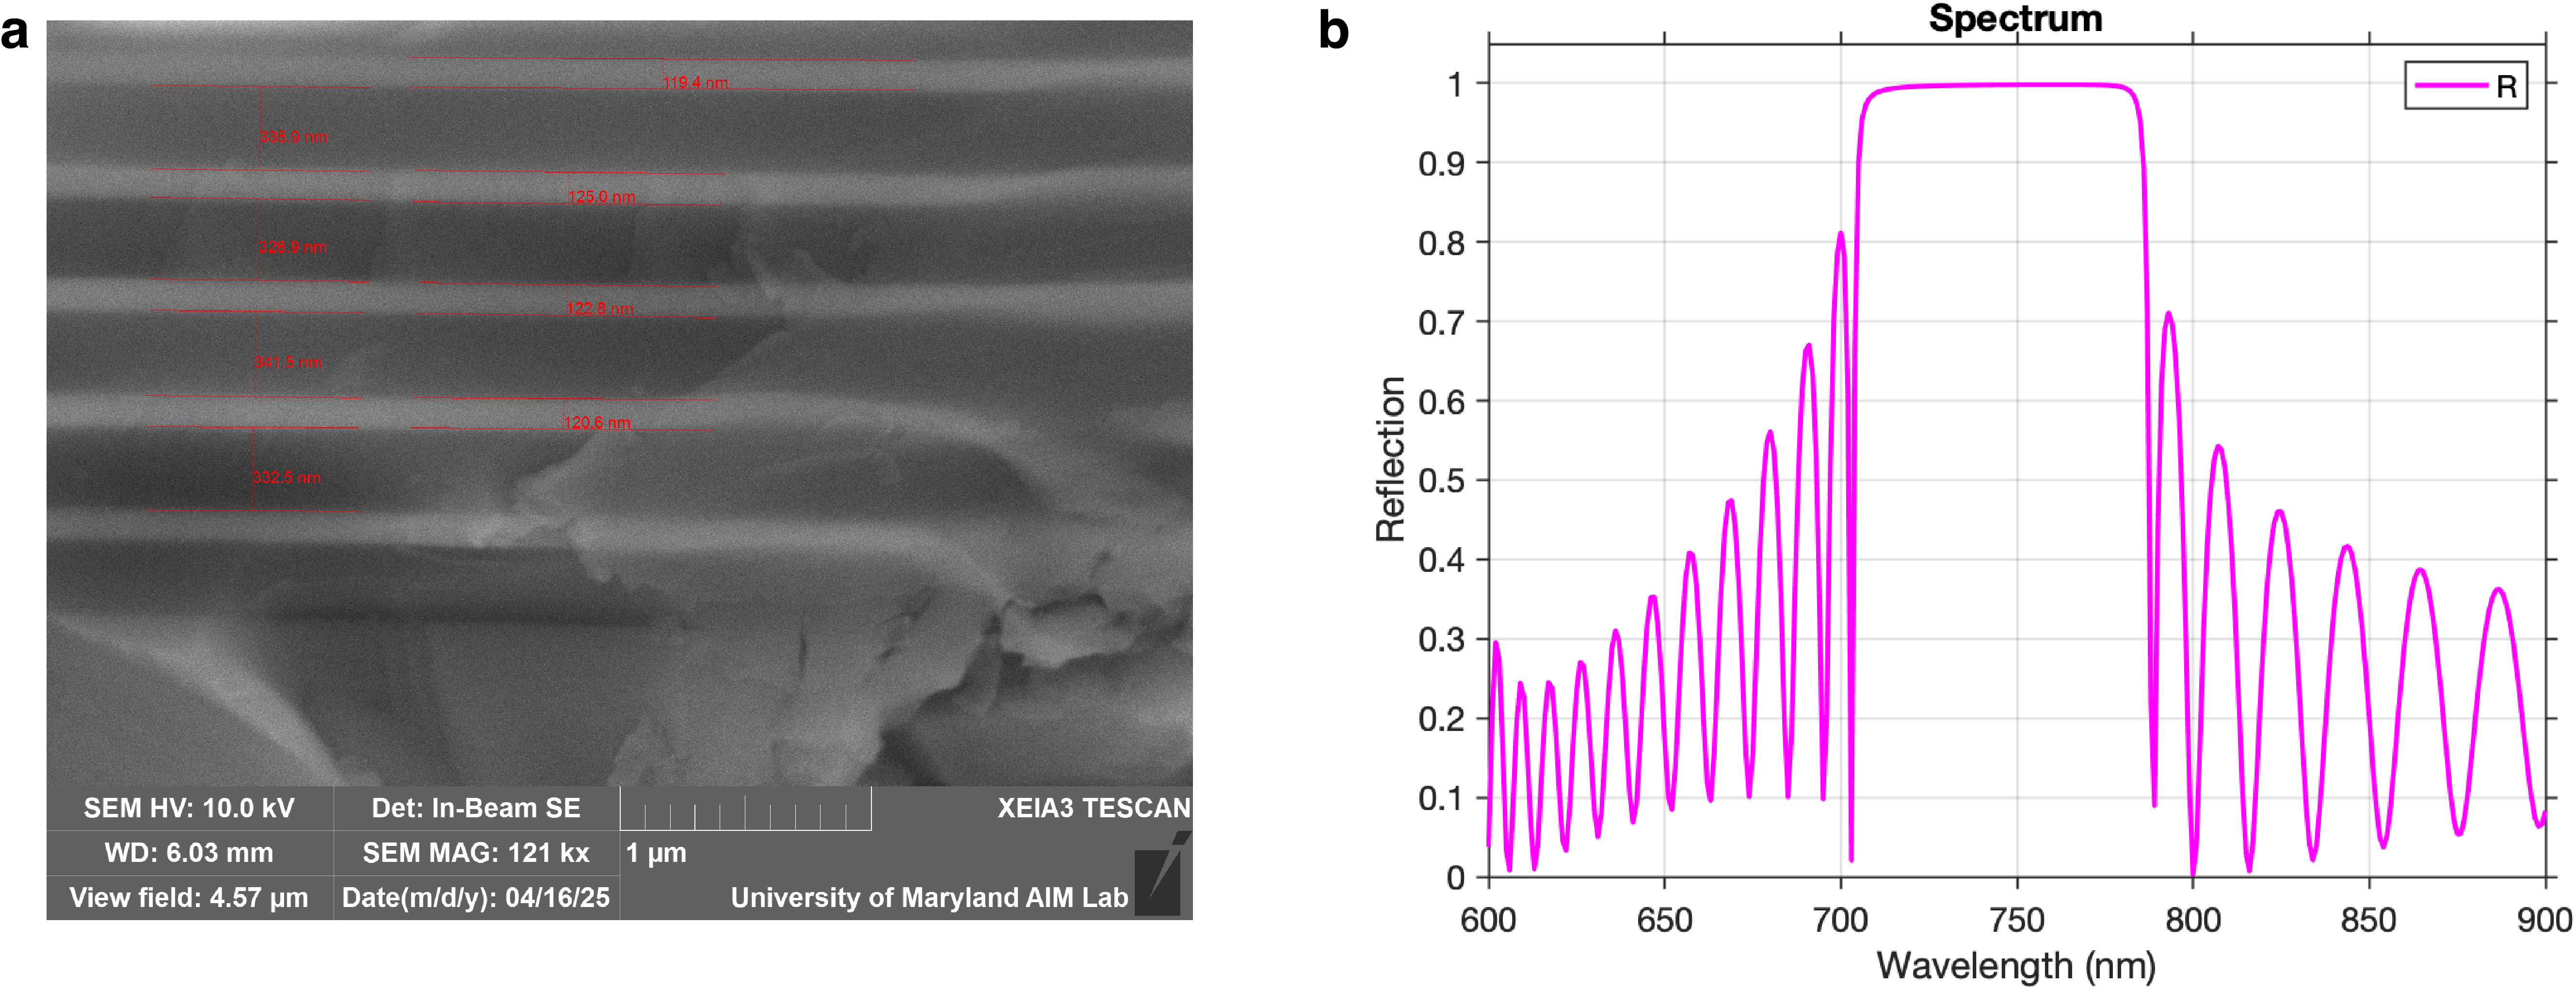
\includegraphics[width=0.9\textwidth]{Figures/C2/Fig.2-5_DBR.jpg} 
\end{center}
\caption[Structure of the sputtered DBR reviled by the cross section SEM and the reflectance spectrum calculated by TMM method.] {Structure of the sputtered DBR reviled by the cross section SEM \textbf{a} and the reflectance spectrum calculated by TMM method \textbf{b}.}
\label{fig.DBR}
\end{figure}
\end{quote}
\renewcommand{\baselinestretch}{2}
\small\normalsize
% --------
The cavity mode with the resonance at $\lambda_0$ can be formed by placing two DBRs with a separation corresponding to an optical thickness of $l_c = n\frac {\lambda}{2 n_0}$. Where $n$ is an integer. 
In this Fabry--P\'erot microcavity, the optical field is confined only in the $z$ direction but free in the $x$--$y$ plane. 
The distribution of the standing wave can be calculated by the transfer matrix method(see in Chapter 3). 

In the 1D microcavity, the cavity photon exhibits an in-plane energy dispersion as a function of the in-plane wavevector $k_{\parallel}$\cite{Deng2010-ul}:
\begin{equation}
E_{\mathrm{cav}} = \frac{\hbar c}{n_c} \sqrt{k_{\parallel}^2 + k_{\perp}^2},
\label{eq:cavity_dispersion}
\end{equation}
\vspace{-0.5em}
where the longitudinal wavevector is 
\vspace{-0.5em}
\begin{equation}
k_{\perp} = \frac{2\pi n_c}{\lambda}.
\label{eq:k_perp}
\end{equation}\vspace{-0.5em}
Given a photon incident angle $\theta$, the in-plane component of the wavevector can be approximated as:
\begin{equation}
k_{\parallel} \approx \frac{2\pi}{\lambda} \, \theta, 
\qquad \text{when } k_{\parallel} \ll k_{\perp}.
\label{eq:k_parallel}
\end{equation}\vspace{-0.5em}
Thus, the cavity energy can be expressed in a parabolic form as
\begin{equation}
E_{\mathrm{cav}} \approx \frac{\hbar c}{n_c} k_{\perp} 
+ \frac{\hbar^2 k_{\parallel}^2}{2 m_{\mathrm{cav}}},
\label{eq:cavity_parabola}
\end{equation}
where $m_{\mathrm{cav}}$ is the effective photon mass of the cavity mode.

\subsection{Strong coupling exciton polaritons}
The fundamental TE mode has its electric field within the cavity plane (transverse to $z$), matching the in-plane transition dipole of bright TMD excitons. 
According to the Fermi’s golden rule, the transition rate $\Gamma_{\omega}$ can be expressed as:
\begin{equation}
\Gamma(\omega)\;\propto\; \big|\langle X|\,(-\mathbf{d}\!\cdot\!\mathbf{E})\,|0\rangle\big|^{2}\,\rho(\omega)
= \big|\mathbf{d}\big|^{2}\,\big|\mathbf{E}\big|^{2}\,\kappa^{2}\,\rho(\omega),
\qquad \kappa \equiv \hat{\mathbf{d}}\!\cdot\!\hat{\mathbf{E}},
\end{equation}
Thus the alignment ($\kappa\!=\!1$) maximizes the $\Gamma$ for the TE mode.
where $\mathbf d$ is the exciton transition dipole, $\mathbf E$ is the cavity field at the monolayer, $\rho(\omega)$ is the photonic density of states, and $\kappa\equiv \hat{\mathbf d}\!\cdot\!\hat{\mathbf E}$ is the polarization (orientation) factor; TE polarization gives $\kappa\simeq 1$, whereas TM fields with an out-of-plane component reduce $\kappa$.
In cavity QED, the vacuum Rabi coupling for a single exciton to the cavity photon can be expressed by the coupling coefficient $g_1$ as:
\begin{equation}
g_1 \;=\; \frac{1}{\hbar}\,\big|\mathbf{d}\!\cdot\!\mathbf{E}_{\rm vac}\big|
\;=\; \frac{|\mathbf{d}|}{\hbar}\,\sqrt{\frac{\hbar\omega_c}{2\varepsilon_0 \varepsilon_b V_{\rm eff}}}\;\kappa,
\end{equation}
where $V_{\rm eff}\!\approx\!A\,L_{\rm eff}$ for a planar cavity, $\varepsilon_b$ is the background permittivity, and $\kappa$ is the polarization (orientation) factor. 
The effective cavity length $L_{\rm eff}$ consist of the cavity spacer length $L_{\rm eff}$ and the field penetration length $L_{\rm DBR}$, which is given by:
\begin{equation}
\ell_{\mathrm{eff}} = \frac{\lambda_0}{2}\,
\frac{n_{\mathrm{1}}\,n_{\mathrm{2}}}{\,n_0\,(\,n_{\mathrm{2}} - n_{\mathrm{2}}\,)} \, 
\end{equation}\vspace{-0.5em}
For the 2D exciton sheet, we assume there are $N$ numbers of exciotns within the mode area and can coherently couple to the cavity mode. 
This collective coupling strength can be expressed as:
\begin{equation}
g_{\rm 0} \;=\; \sqrt{N}\,g_1 \;\;\Rightarrow\;\;
\hbar\Omega_R \;=\; 2 g_{\rm 0}
\end{equation}\vspace{-0.5em}
The resulting hybrid light–matter quasiparticles are cavity polaritons. 
And when we looking at the exciton-polairton Hamiltonian, the microscopic coupling $g_{\rm 0}$ appears as the off-diagonal term at fixed in-plane wavevector $k_{\parallel}$:
\begin{equation}
\begin{aligned}
\hat H_{\mathrm{pol}}
&= \hat H_{\mathrm{cav}}+\hat H_{\mathrm{exc}}+\hat H_{\mathrm{int}} \\
&= \sum\!\
  E_{\mathrm{cav}}(k_\parallel)\,\hat a_{k_\parallel}^{\dagger}\hat a_{k_\parallel}
 +\sum\!\
  E_{\mathrm{exc}}(k_\parallel)\,\hat b_{k_\parallel}^{\dagger}\hat b_{k_\parallel}
 +\sum\!\
  g_0\big(\hat a_{k_\parallel}^{\dagger}\hat b_{k_\parallel}
         +\hat b_{k_\parallel}^{\dagger}\hat a_{k_\parallel}\big)
\end{aligned}\
\label{eq:H_polariton}
\end{equation}
where $\hat{a}^{\dagger}_{k_{\parallel}}$ ($\hat{b}^{\dagger}_{k_{\parallel}}$) creates a cavity photon (exciton) with in-plane wavevector $k_{\parallel}$, $E_{\mathrm{cav}}(k_{\parallel})$ and $E_{\mathrm{exc}}(k_{\parallel})$ are the bare dispersions, and $g_0$ is the light–matter coupling strength (enhanced by the cavity field and the excitonic oscillator strength).

In the strong-coupling regime (i.e., when the coherent coupling $g_0$ exceeds the relevant photon and exciton dissipation rates), the eigenmodes are coherent superpositions of the bare photon and exciton. 
The transformation to the lower/upper polariton operators is given by the Hopfield mixing:
\begin{equation}
\begin{pmatrix}
\hat{p}_{k_{\parallel}} \\
\hat{q}_{k_{\parallel}}
\end{pmatrix}
=
\begin{pmatrix}
C_{k_{\parallel}} & X_{k_{\parallel}} \\
X_{k_{\parallel}} & -\,C_{k_{\parallel}}
\end{pmatrix}
\begin{pmatrix}
\hat{a}_{k_{\parallel}} \\
\hat{b}_{k_{\parallel}}
\end{pmatrix},
\qquad
|C_{k_{\parallel}}|^{2}+|X_{k_{\parallel}}|^{2}=1,
\label{eq:Hopfield}
\end{equation}
where $|C_{k_{\parallel}}|^{2}$ and $|X_{k_{\parallel}}|^{2}$ quantify the photonic and excitonic fractions, respectively. It can be defined as:
\begin{equation}\
\lvert X_{k_\parallel}\rvert^{2}
= \frac{1}{2}\!\left(
1 + \frac{\Delta E(k_\parallel)}{\sqrt{[\Delta E(k_\parallel)]^{2}+4 g_0^{2}}}
\right)
\end{equation}

\begin{equation}\
\lvert C_{k_\parallel}\rvert^{2}
= \frac{1}{2}\!\left(
1 - \frac{\Delta E(k_\parallel)}{\sqrt{[\Delta E(k_\parallel)]^{2}+4 g_0^{2}}}
\right)
\end{equation}
Diagonalizing Eq.~\eqref{eq:H_polariton} yields the lower (LP) and upper (UP) polariton energies:
\begin{equation}
E_{\mathrm{LP,UP}}(k_{\parallel})
=
\frac{E_{\mathrm{cav}}(k_{\parallel}) + E_{\mathrm{exc}}(k_{\parallel})}{2}
\;\pm\;
\frac{1}{2}\sqrt{\big[E_{\mathrm{cav}}(k_{\parallel}) - E_{\mathrm{exc}}(k_{\parallel})\big]^2 + 4 g_0^{\,2}}\, 
\label{eq:LP_UP}
\end{equation}
From this we can see that when the cavity is on resonance with the exciton frequency (zero detuning), the energy splitting between the lower and upper polariton branch would be $2g_0$. This is also called the vacuum Rabi splitting.
The detuning between the uncoupled modes is defined as:
\begin{equation}
\Delta(k_{\parallel}) \;\equiv\; E_{\mathrm{cav}}(k_{\parallel}) - E_{\mathrm{exc}}(k_{\parallel}) .
\label{eq:detuning}
\end{equation}
At zero detuning ($\Delta=0$),the polaritons are half-light, half-matter ($|C_{k_{\parallel}}|^{2}=|X_{k_{\parallel}}|^{2}=1/2$).
%Fig.1-4--------------
\renewcommand{\baselinestretch}{1}
\small\normalsize
\begin{quote}
\begin{figure}
\begin{center}
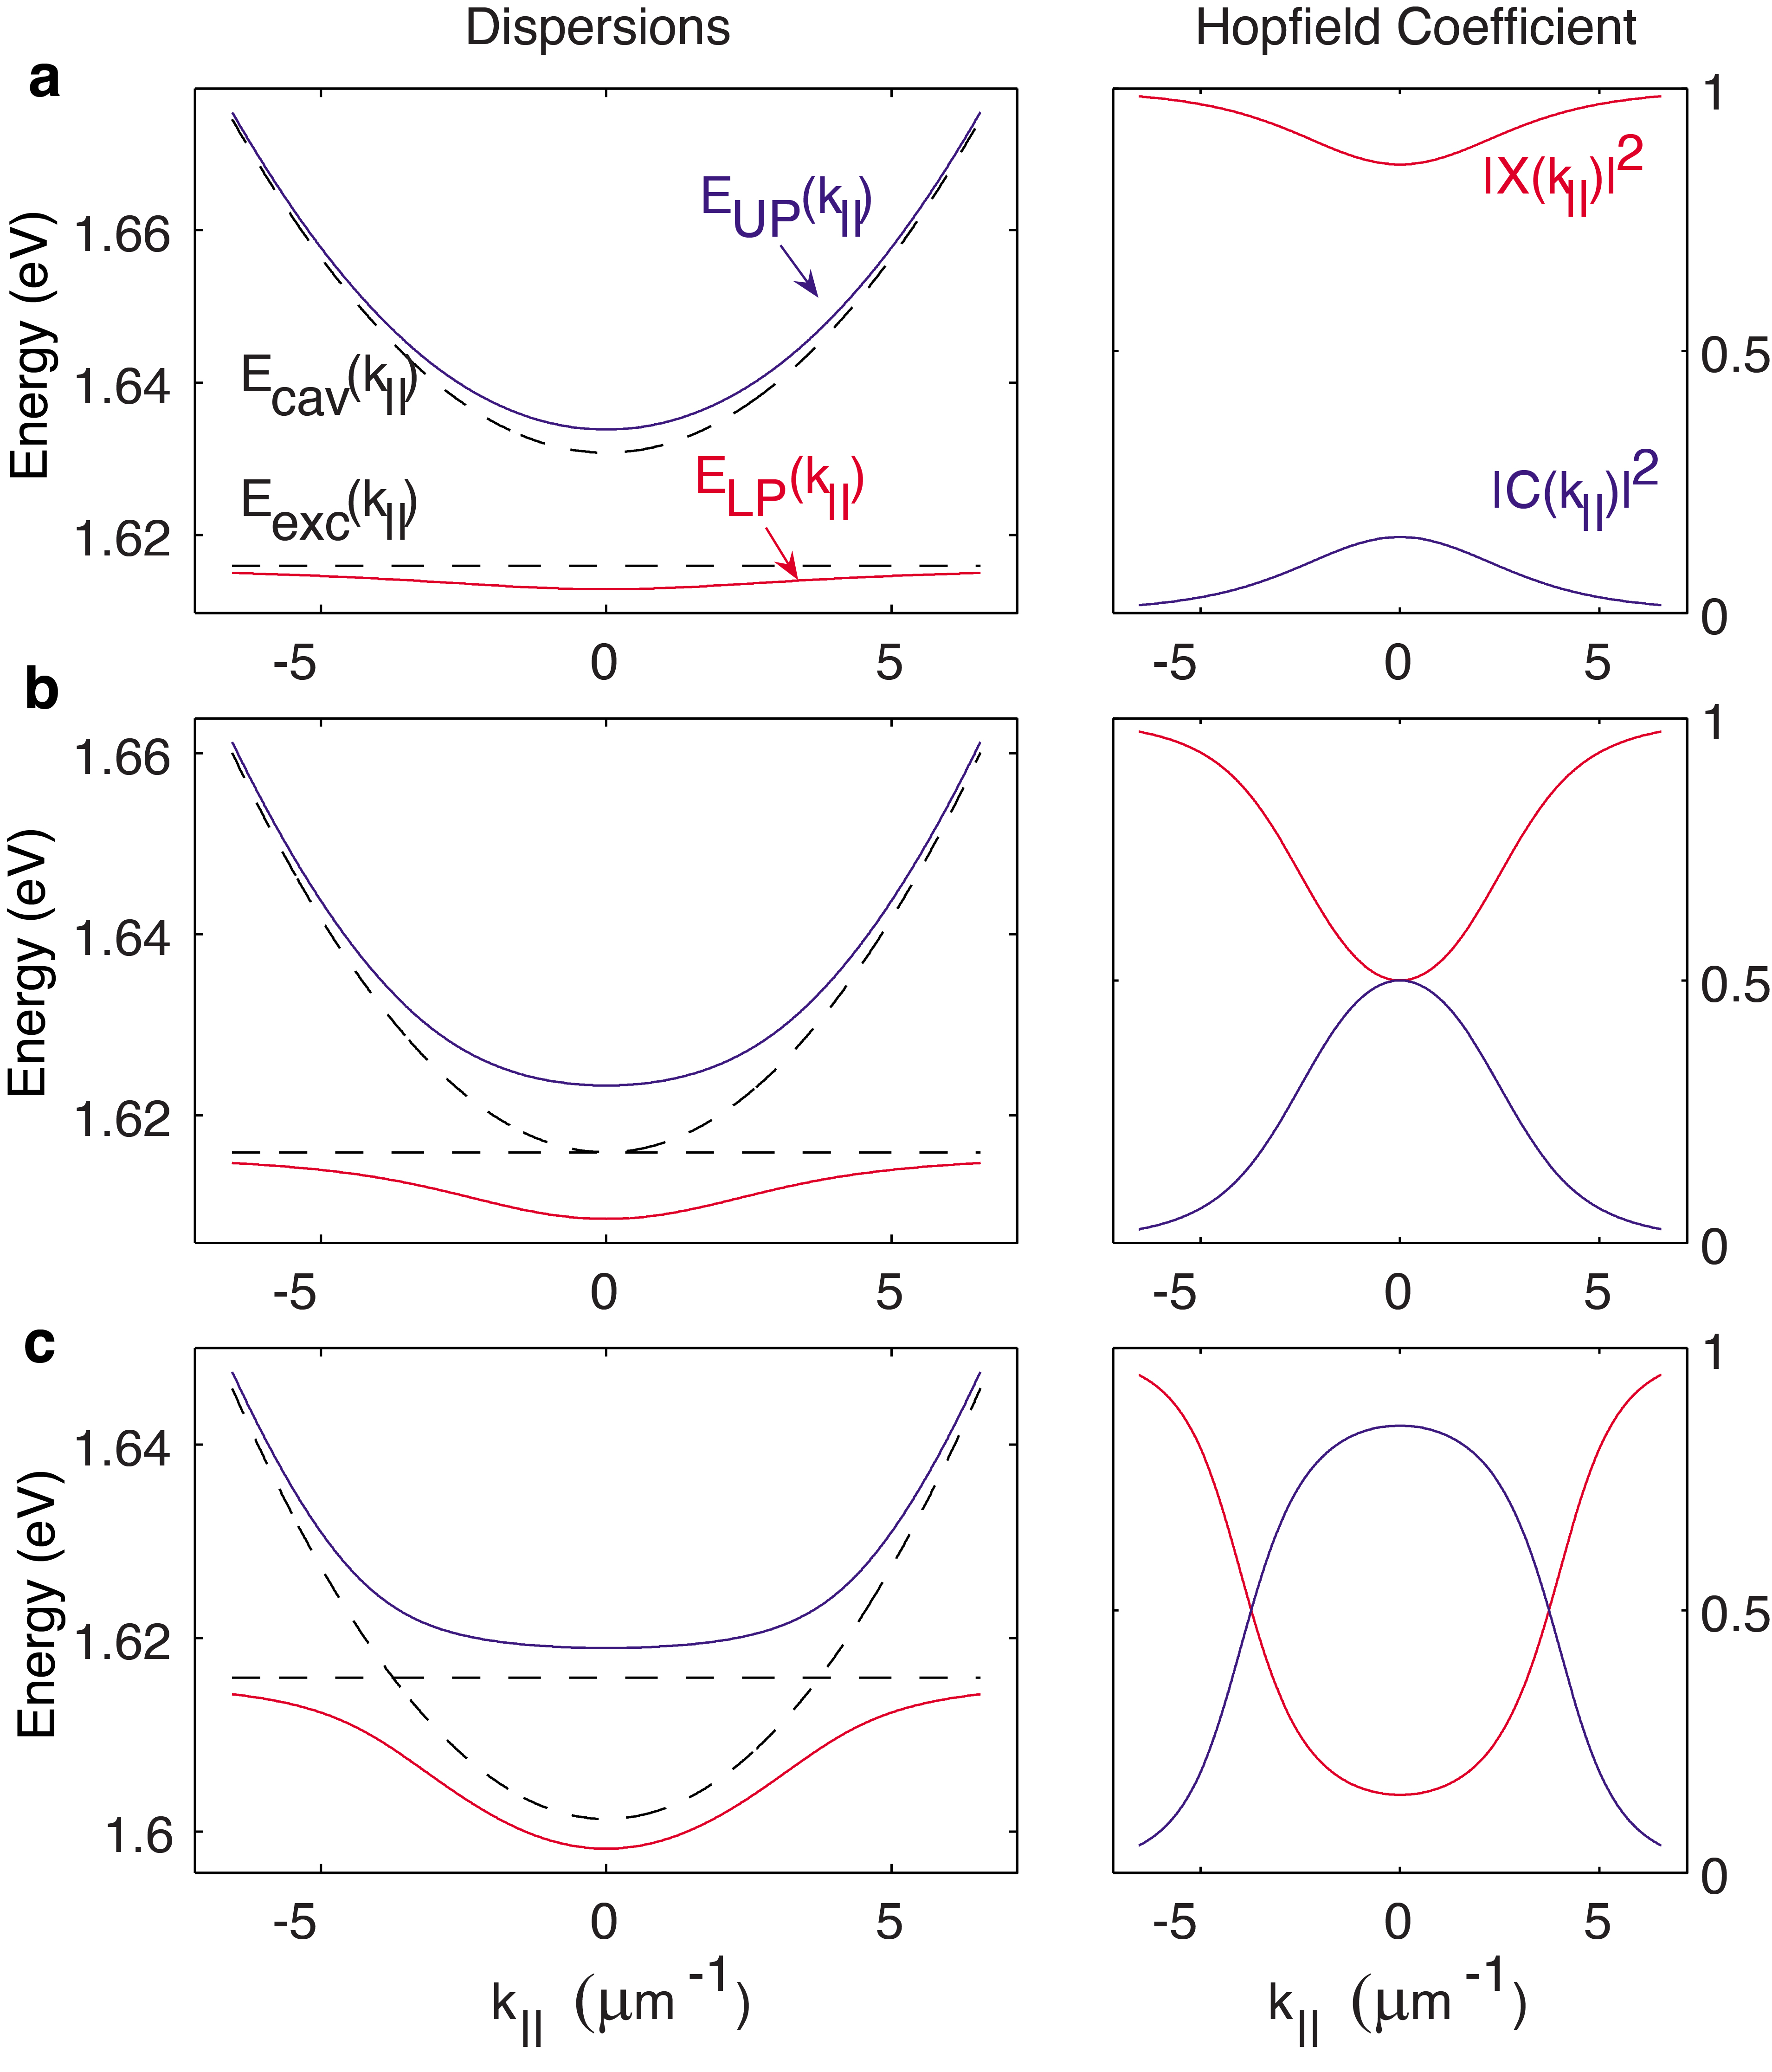
\includegraphics[width=0.8\textwidth]{Figures/C2/Fig.2-6_polariton_detune.jpg} % 
\end{center}
\caption[Exciton polariton dispersions and the Hopfield coefficent for lower polariton at different detuning $\Delta$] {\textbf{Exciton polariton dispersions and the Hopfield coefficent for lower polariton at different detunings.} \textbf{a,} $\Delta= 2 g_0$; \textbf{b,} $\Delta\ = 0$; \textbf{c,} $\Delta\ = -2g_0$.
Figures are adpated from[].}
\label{fig.rydberg_Ex}
\end{figure}
\end{quote}
\renewcommand{\baselinestretch}{2}
\small\normalsize
% --------------
Equivalently, using the 2D oscillator strength per area $f_{2\mathrm{D}}$, we can have the Rabi splitting as:
\begin{equation}
\Omega_R^{2} \;\propto\; \frac{f_{2\mathrm{D}}}{\varepsilon_b\,L_{\rm eff}}\,\kappa^{2}
\end{equation}
This shows that the in-plane TE polarization ($\kappa\!\approx\!1$) maximizes $\Omega_R$, and larger $f_{2\mathrm{D}}$ and smaller $L_{\rm eff}$ would further increase the Rabi splitting. 
Since the planar (1D) cavity provides an in-plane TE field aligned to the TMD intralayer exciton dipole, the dipole–field overlap $\lvert\mathbf d\!\cdot\!\mathbf E\rvert$ is maximized. 
Leveraging the monolayer’s large oscillator strength and the enhancement at the field antinode, the strong coupling regime is easy to access in the TMD embedded microcavity system, even with limited quality factor. 
The strong coupling is obtained when
\begin{equation}
2 g_{\rm 0} \;>\; \frac{1}{2}\big(\gamma_{\rm cav} + \gamma_{exciton}\big)
\end{equation}
where $\gamma_{\rm cav}$ and $\gamma_{exciton}$ are the cavity and exciton linewidths.
% \smallskip



\titleformat{\chapter}
{\normalfont\large}{Appendix \thechapter:}{1em}{}
%\include{AppendixA}

\renewcommand{\baselinestretch}{1}
\small\normalsize

\addcontentsline{toc}{chapter}{Bibliography}
\include{Bibliography} %To be used when typing your own bibliography
\bibliographystyle{unsrt}

\end{document}
